\section{Simulation Studies}

\begin{frame}
\frametitle{Robot Planner 1: Simple MoveIt planning}
\textbf{Goal}: Benchmark MoveIt Path planning algorithms
\begin{center}
\begin{figure}[!htb]
\centering
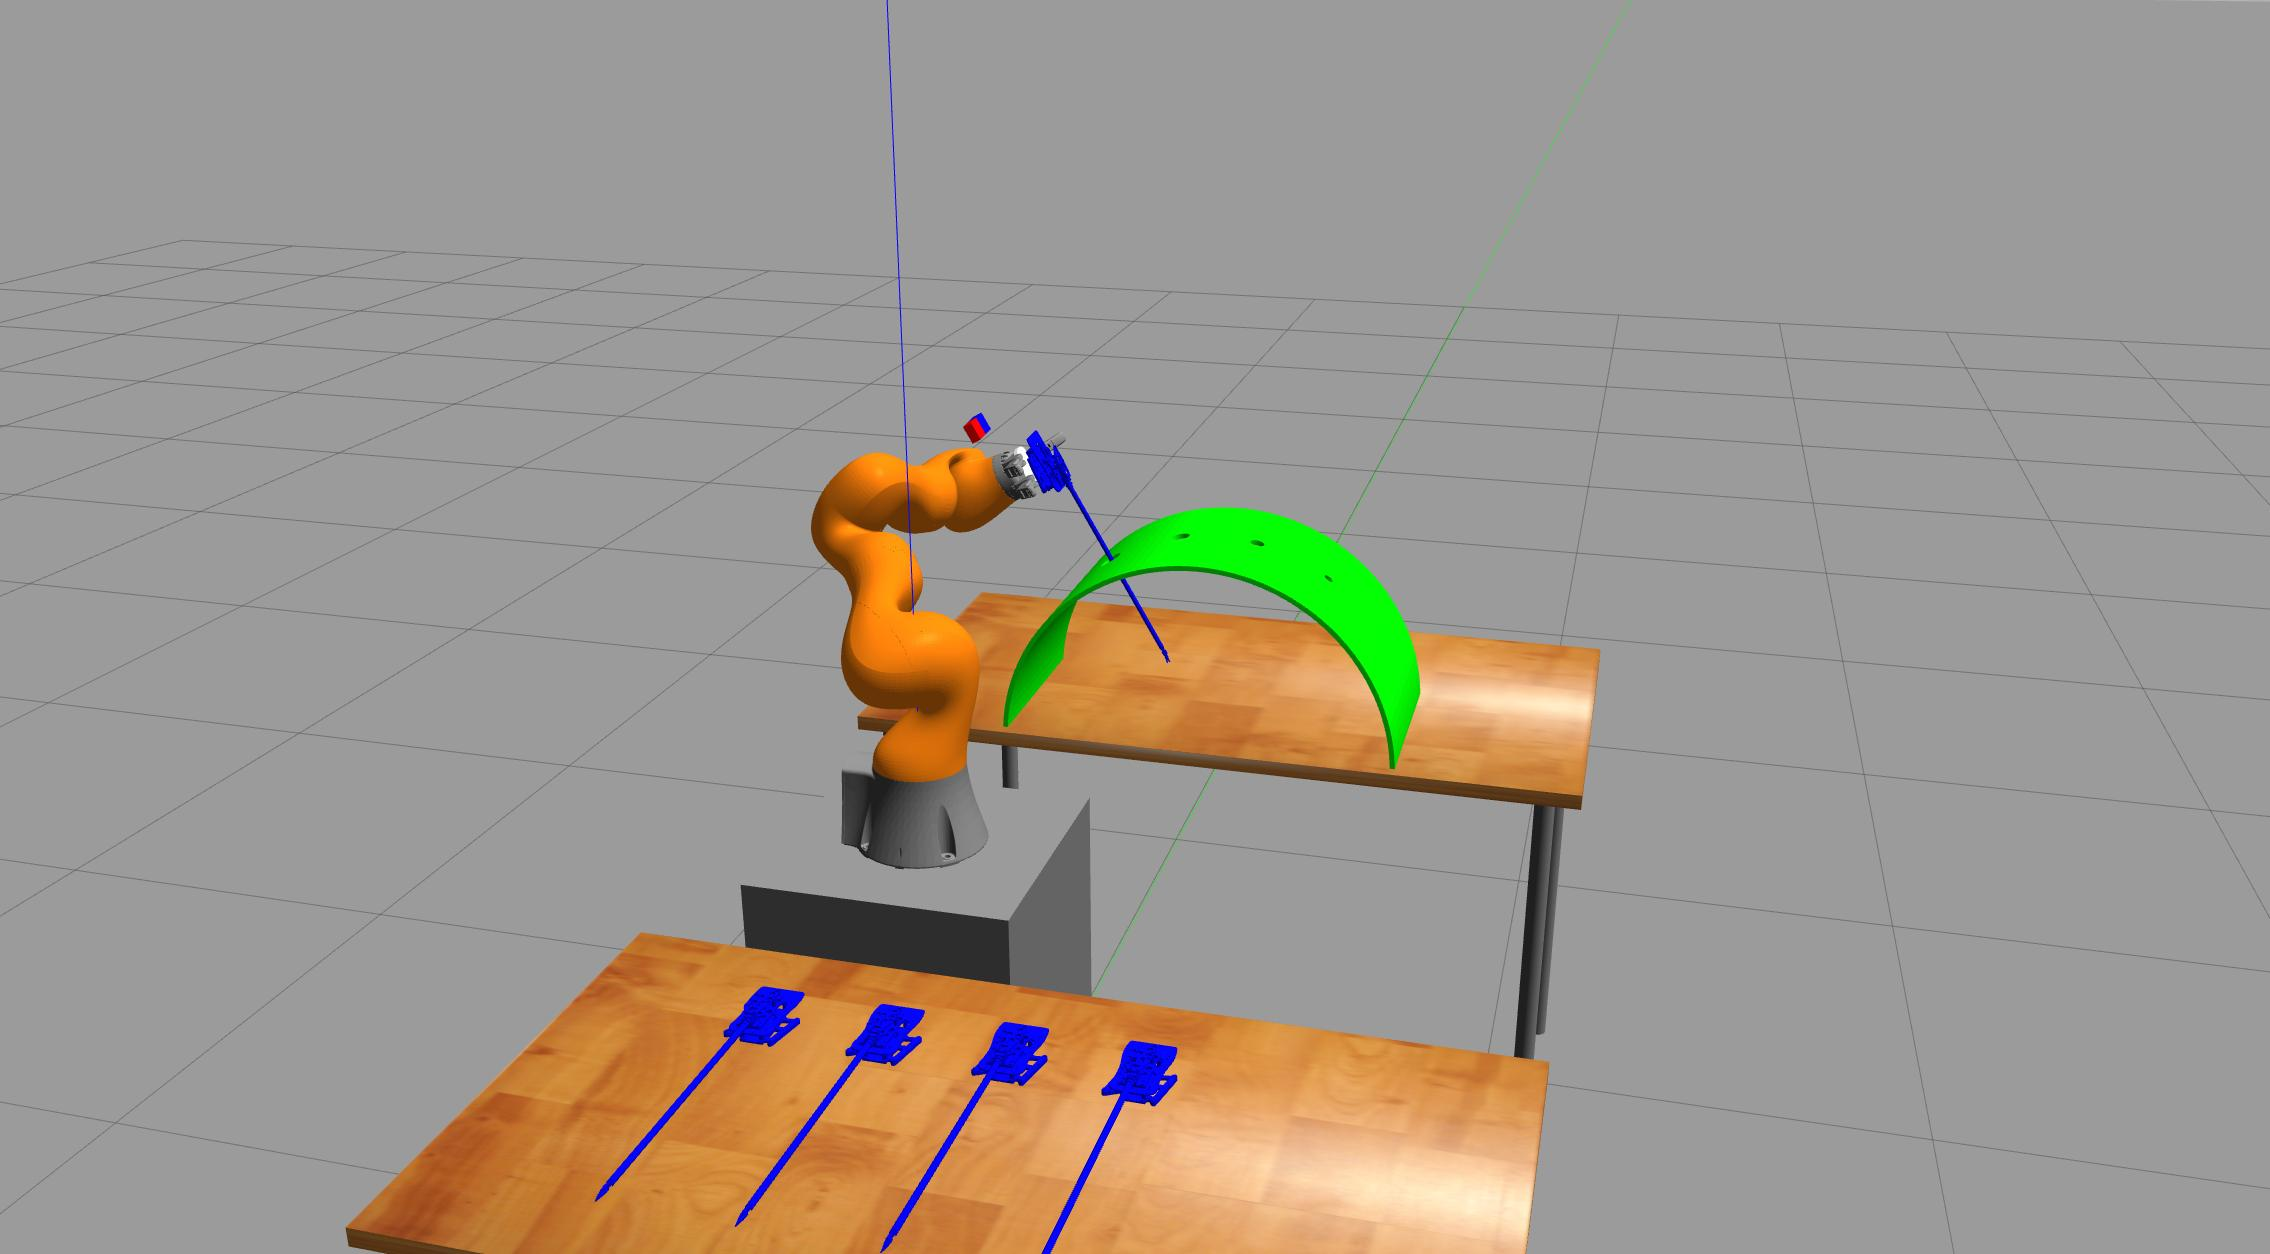
\includegraphics[width=0.9\textwidth]{../images/robot_planner1/robot_planner1_5.jpg}
\end{figure}
\end{center}
\end{frame}

\begin{frame}
\frametitle{Robot Planner 1: Simple MoveIt planning}
\resizebox*{\textwidth}{!}{
\begin{tabular}{|p{2cm}|c|p{2cm}|p{2cm}|p{2cm}|}
\hline
               & \multicolumn{4}{c}{\textbf{RRTConnect}}                                                                                                 \vline \\
\hline
               & \multicolumn{4}{c}{\textbf{Insertion \& Pivot trajectories}}                     \vline \\
\hline
10 Experiments & Insertion planning time & Execution status & Pivot planning time & Execution status  \\
\hline
\textbf{Average} & 	0.163102 & 1	& 0.5014398 &	0.9 \\
\hline
\textbf{Standard deviation} & 	0.110001 &	- &	1.110582 & - \\
\hline
\end{tabular}
}

\resizebox*{\textwidth}{!}{
\begin{tabular}{|p{2cm}|c|p{2cm}|p{2cm}|p{2cm}|}
\hline
               & \multicolumn{4}{c}{\textbf{RRT*}}                                                                                                 \vline \\
\hline
               & \multicolumn{4}{c}{\textbf{Insertion \& Pivot trajectories}}                     \vline \\
\hline
10 Experiments & Insertion planning time & Execution status & Pivot planning time & Execution status  \\
\hline
\textbf{Average} & 	5.083449	& 0.9	& 5.090813	& 0.6 \\
\hline
\textbf{Standard deviation} & 	0.066253 &	- &	0.041338 & - \\
\hline
\end{tabular}
}
\end{frame}


\begin{frame}
\frametitle{Robot Planner 2: Simulation layout and reachability experiments}
\begin{center}
\textbf{Goal}: Find layout with better reachability
\begin{figure}[!htb]
\centering
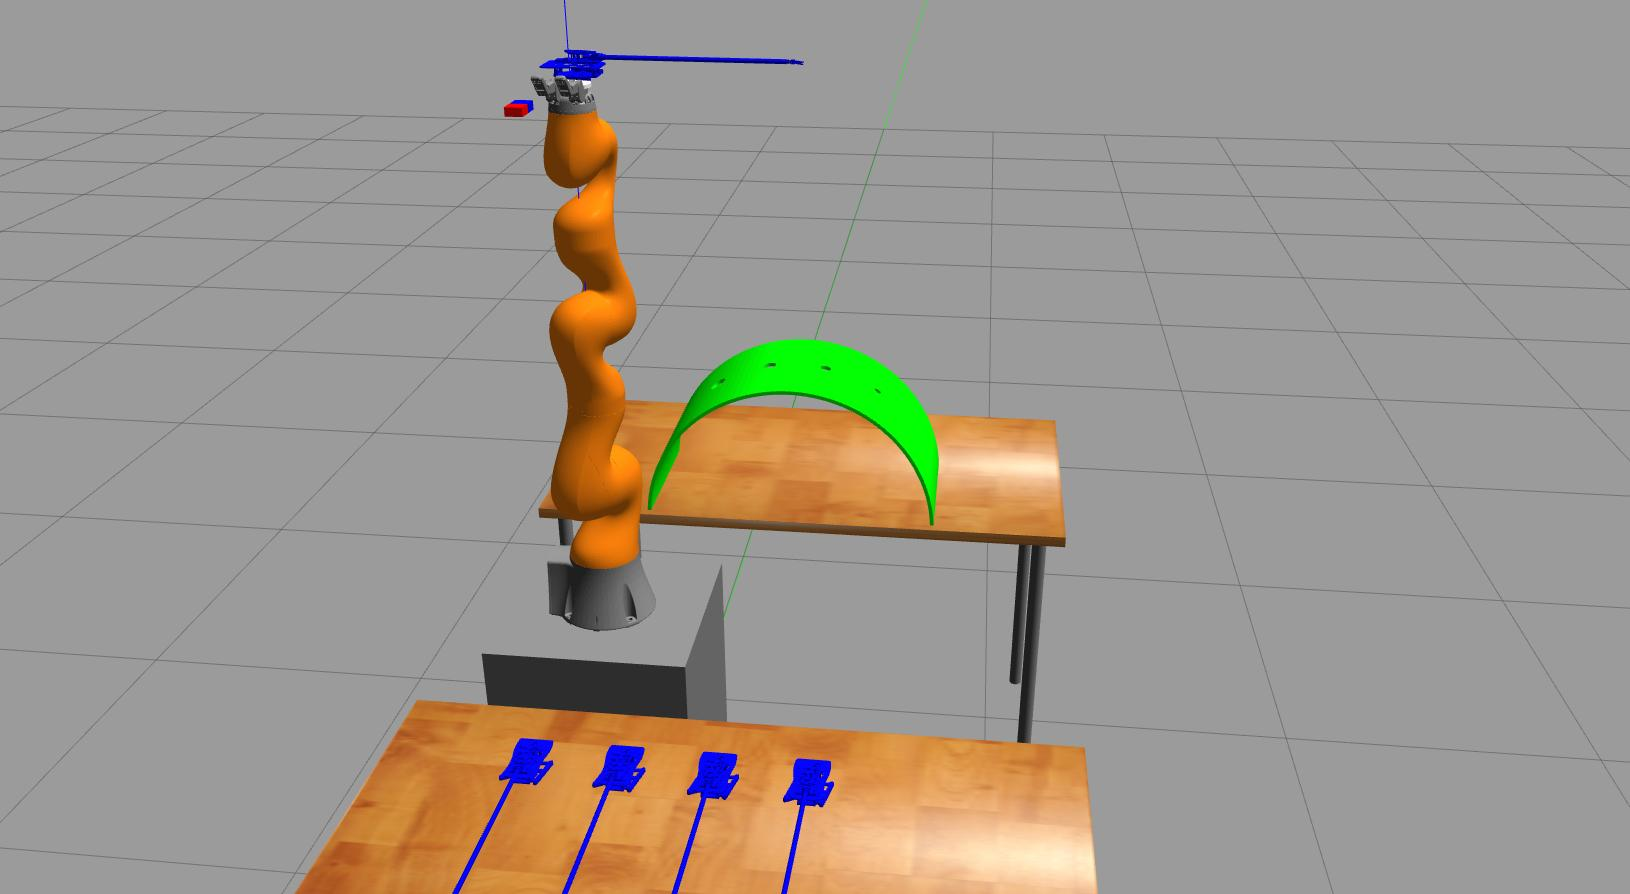
\includegraphics[width=0.3\textwidth]{../images/robot_planner2/robot_planner2_1}
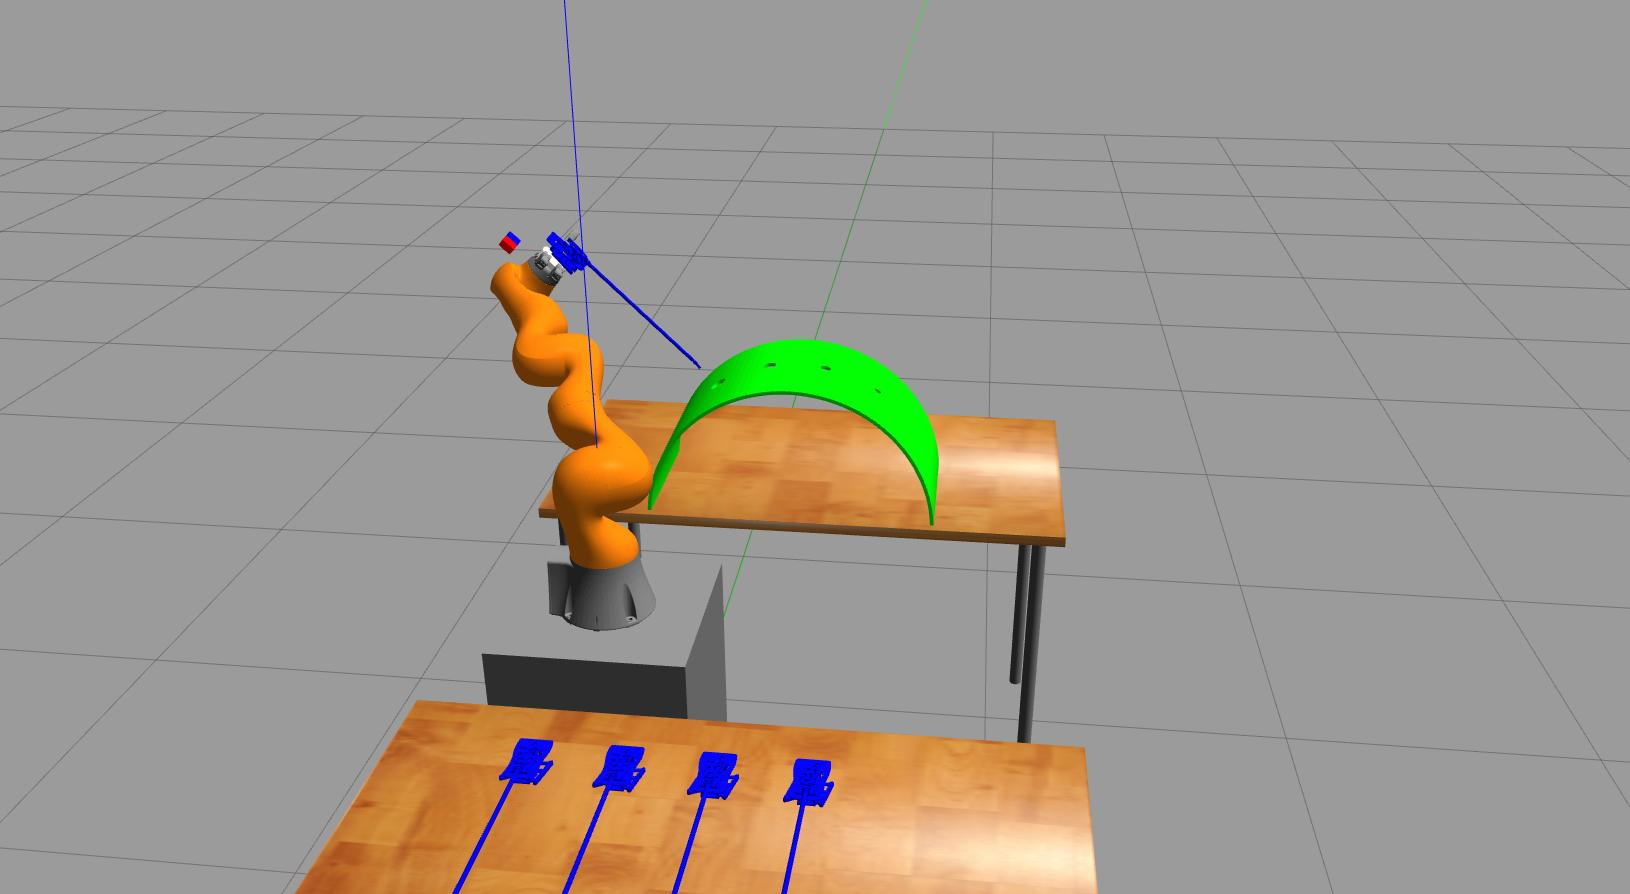
\includegraphics[width=0.3\textwidth]{../images/robot_planner2/robot_planner2_2}
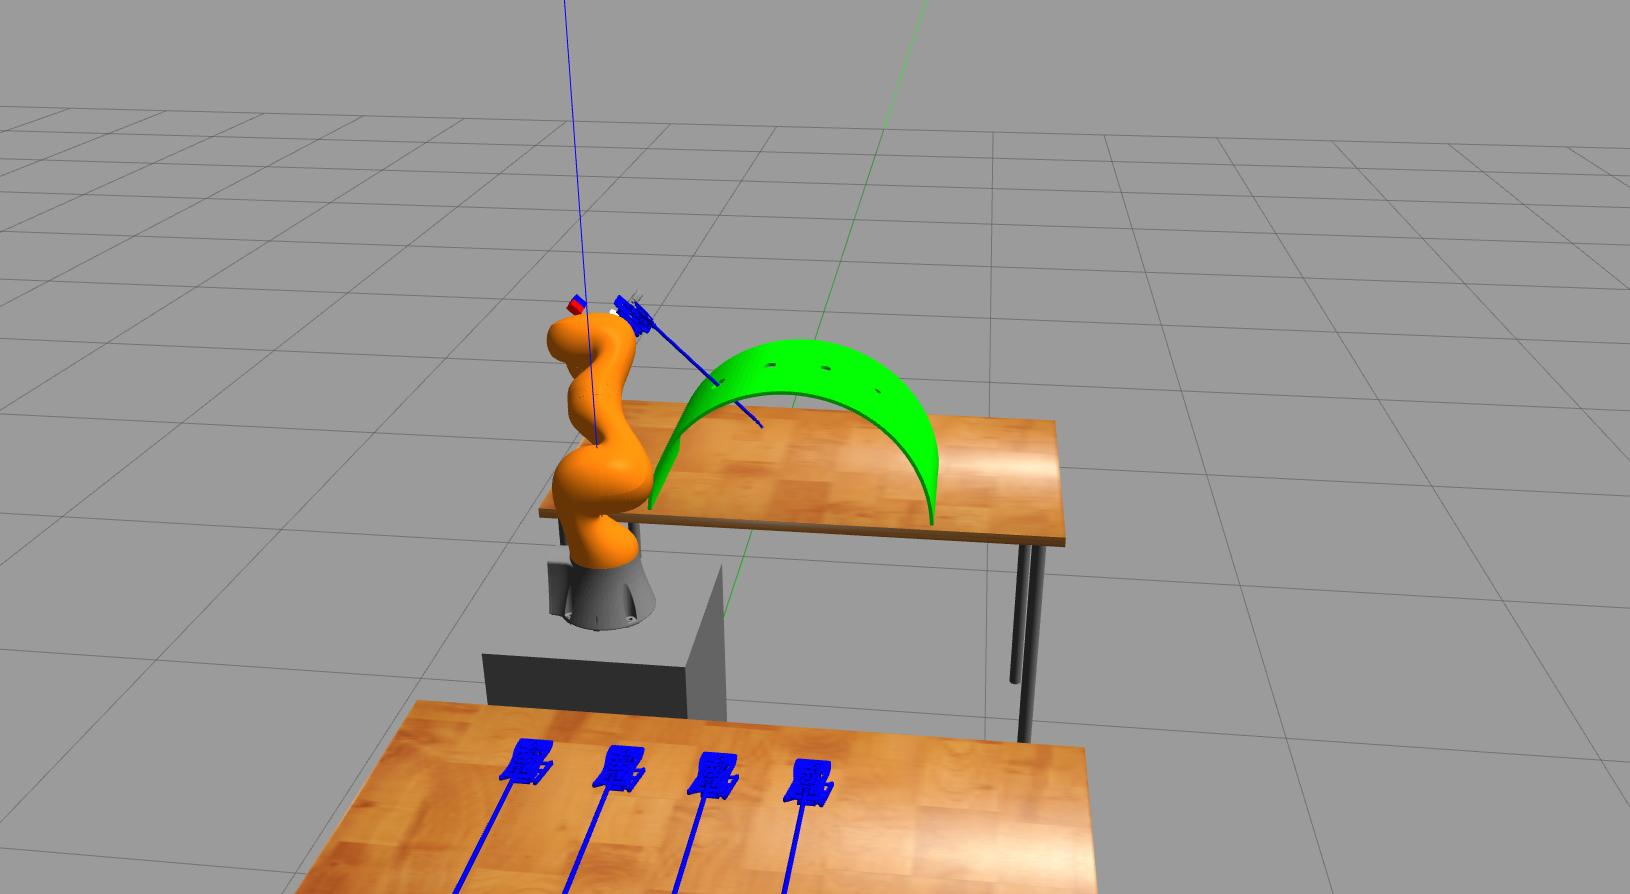
\includegraphics[width=0.3\textwidth]{../images/robot_planner2/robot_planner2_3}\\
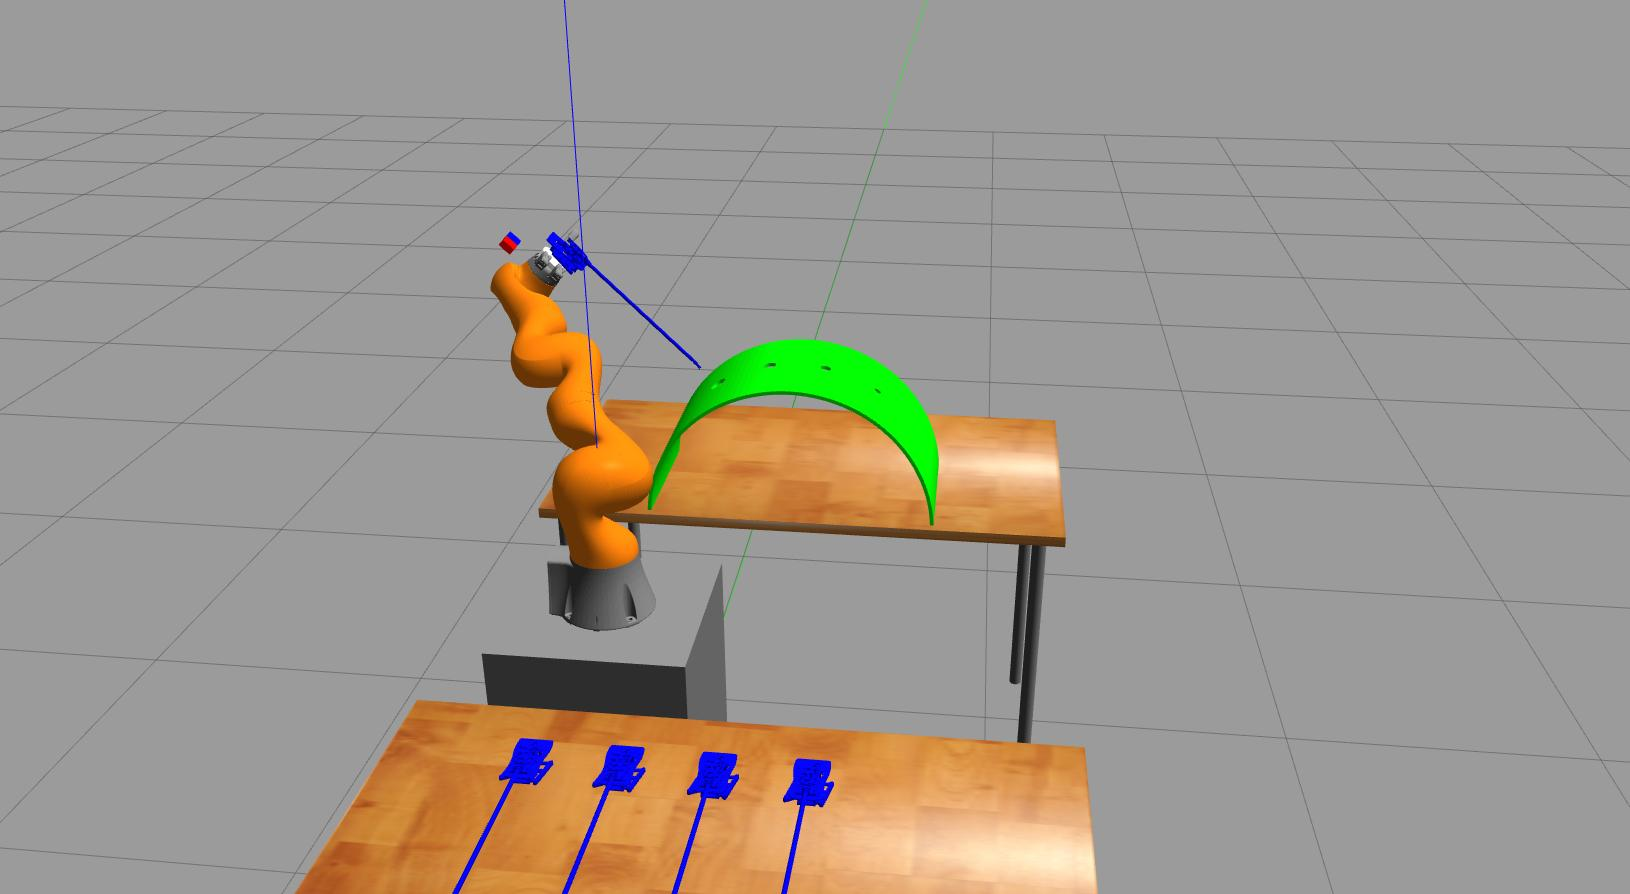
\includegraphics[width=0.3\textwidth]{../images/robot_planner2/robot_planner2_4}
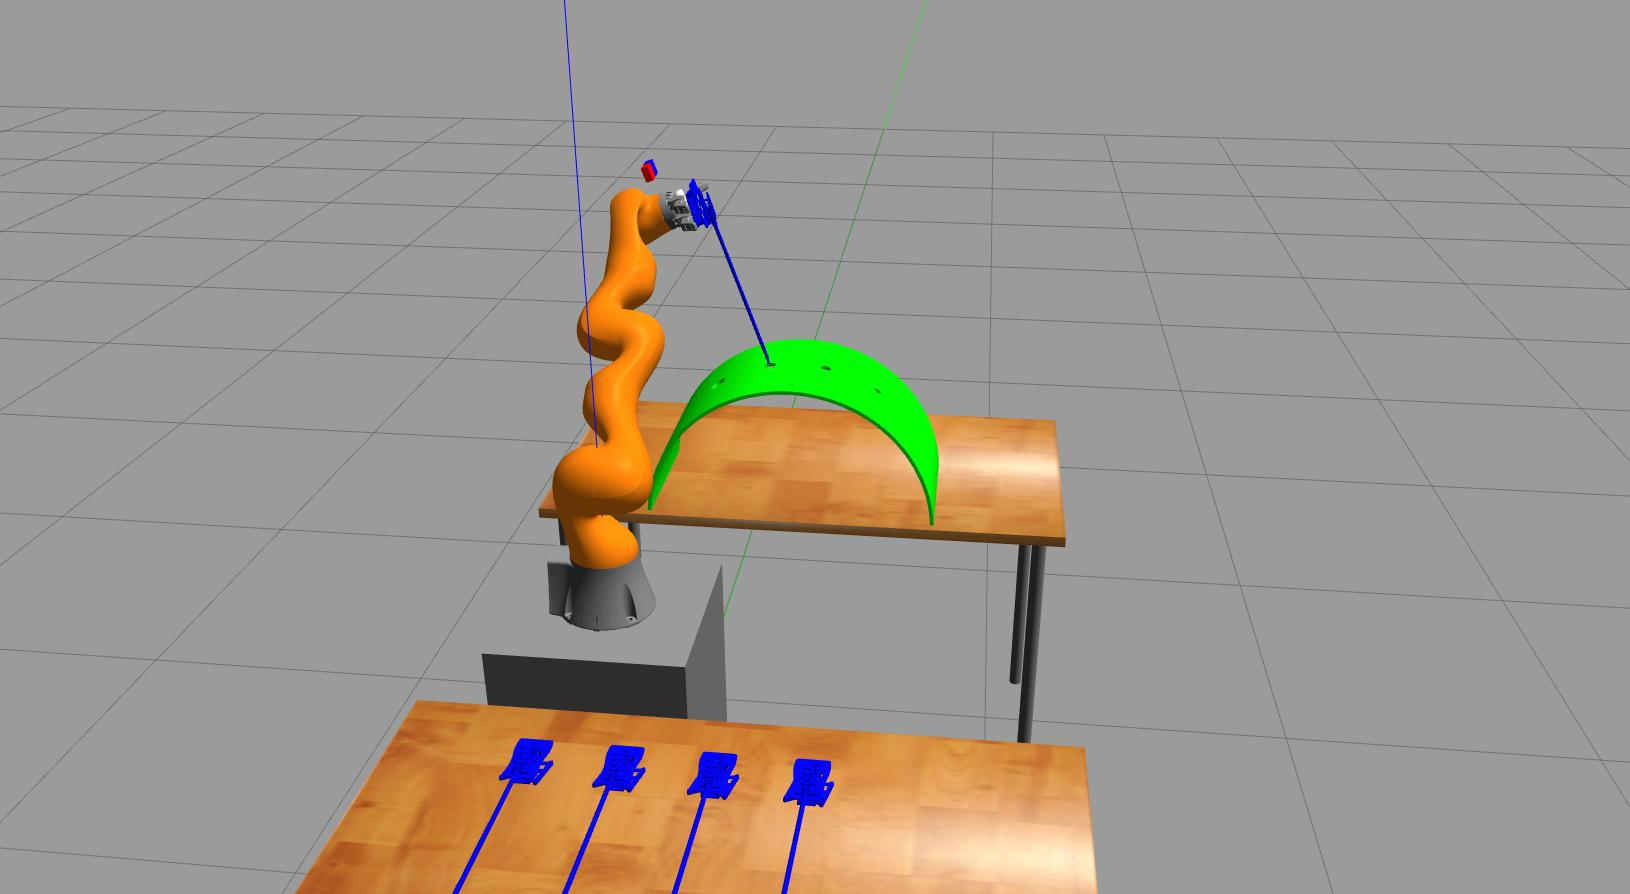
\includegraphics[width=0.3\textwidth]{../images/robot_planner2/robot_planner2_5}
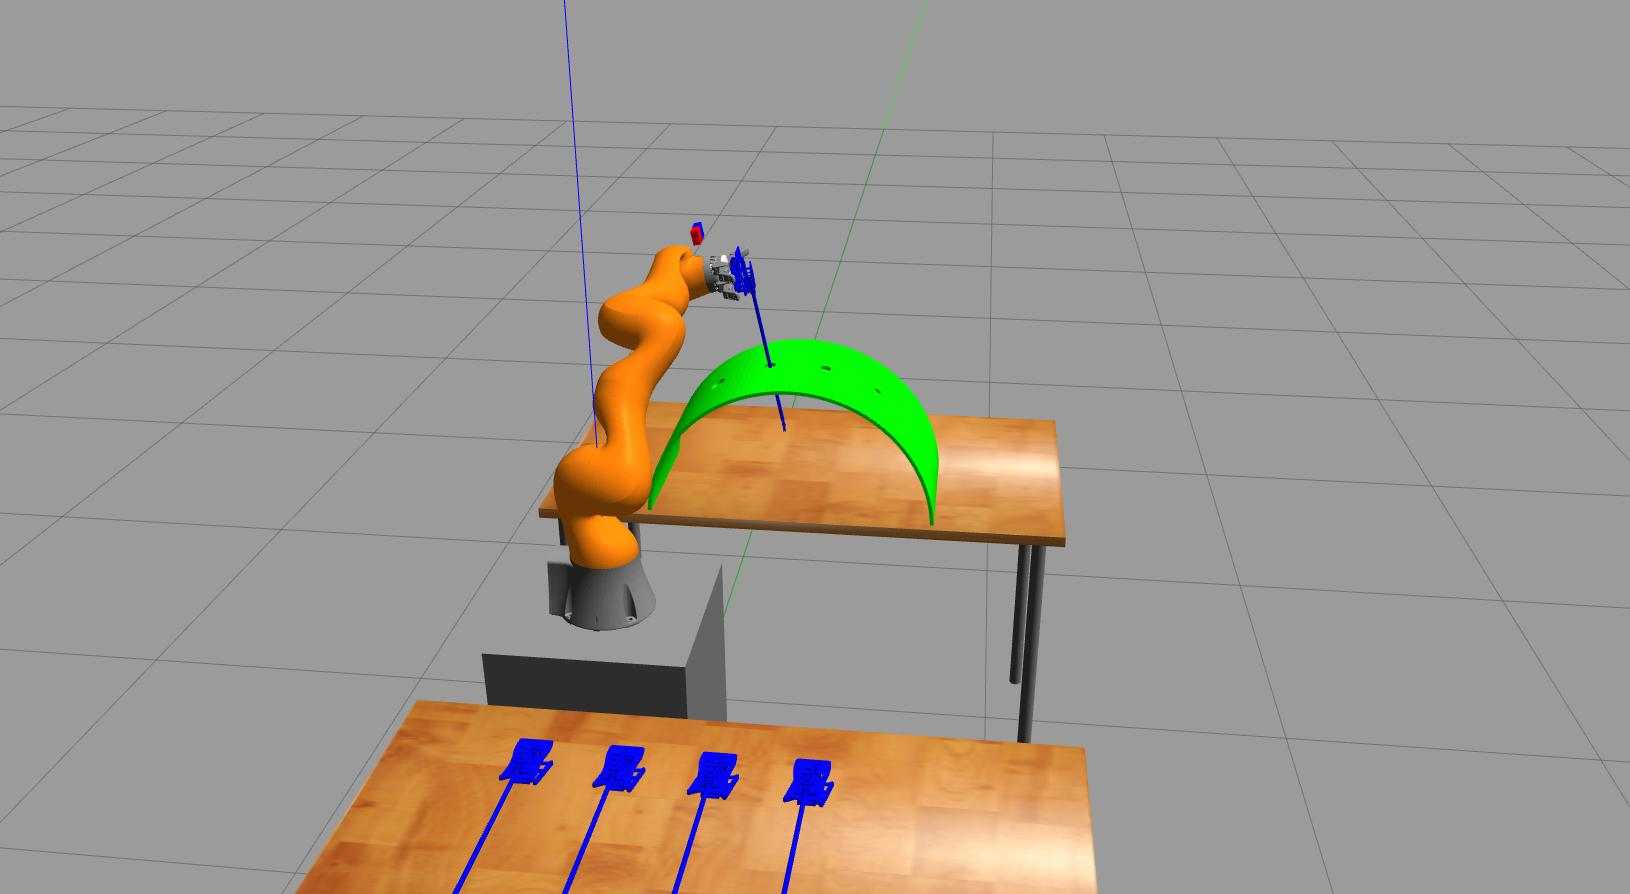
\includegraphics[width=0.3\textwidth]{../images/robot_planner2/robot_planner2_6}\\
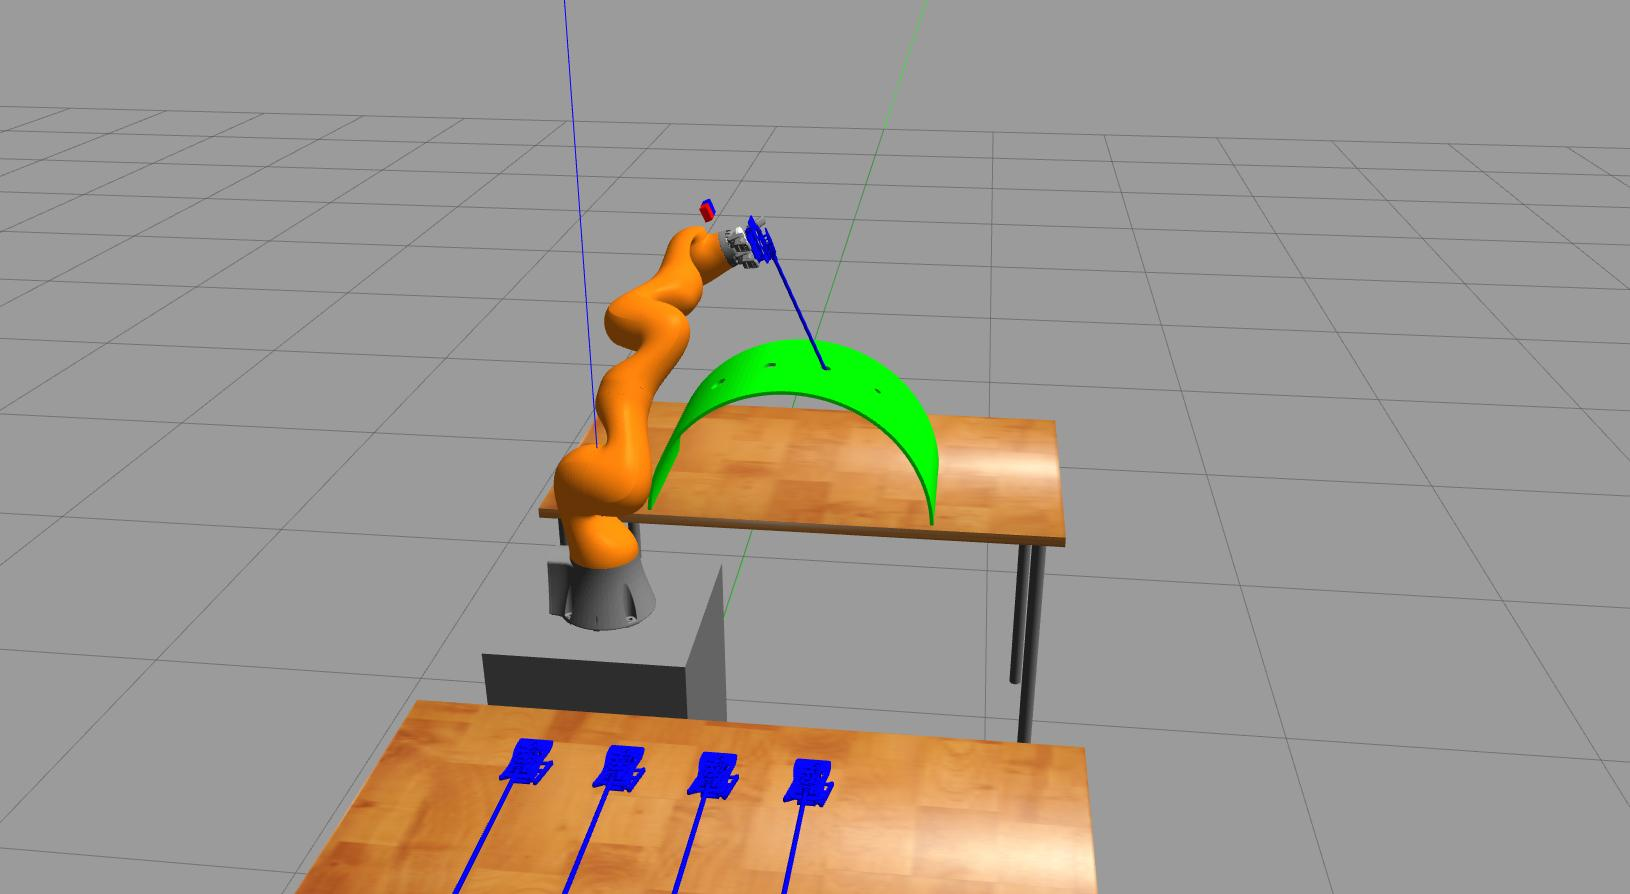
\includegraphics[width=0.3\textwidth]{../images/robot_planner2/robot_planner2_7}
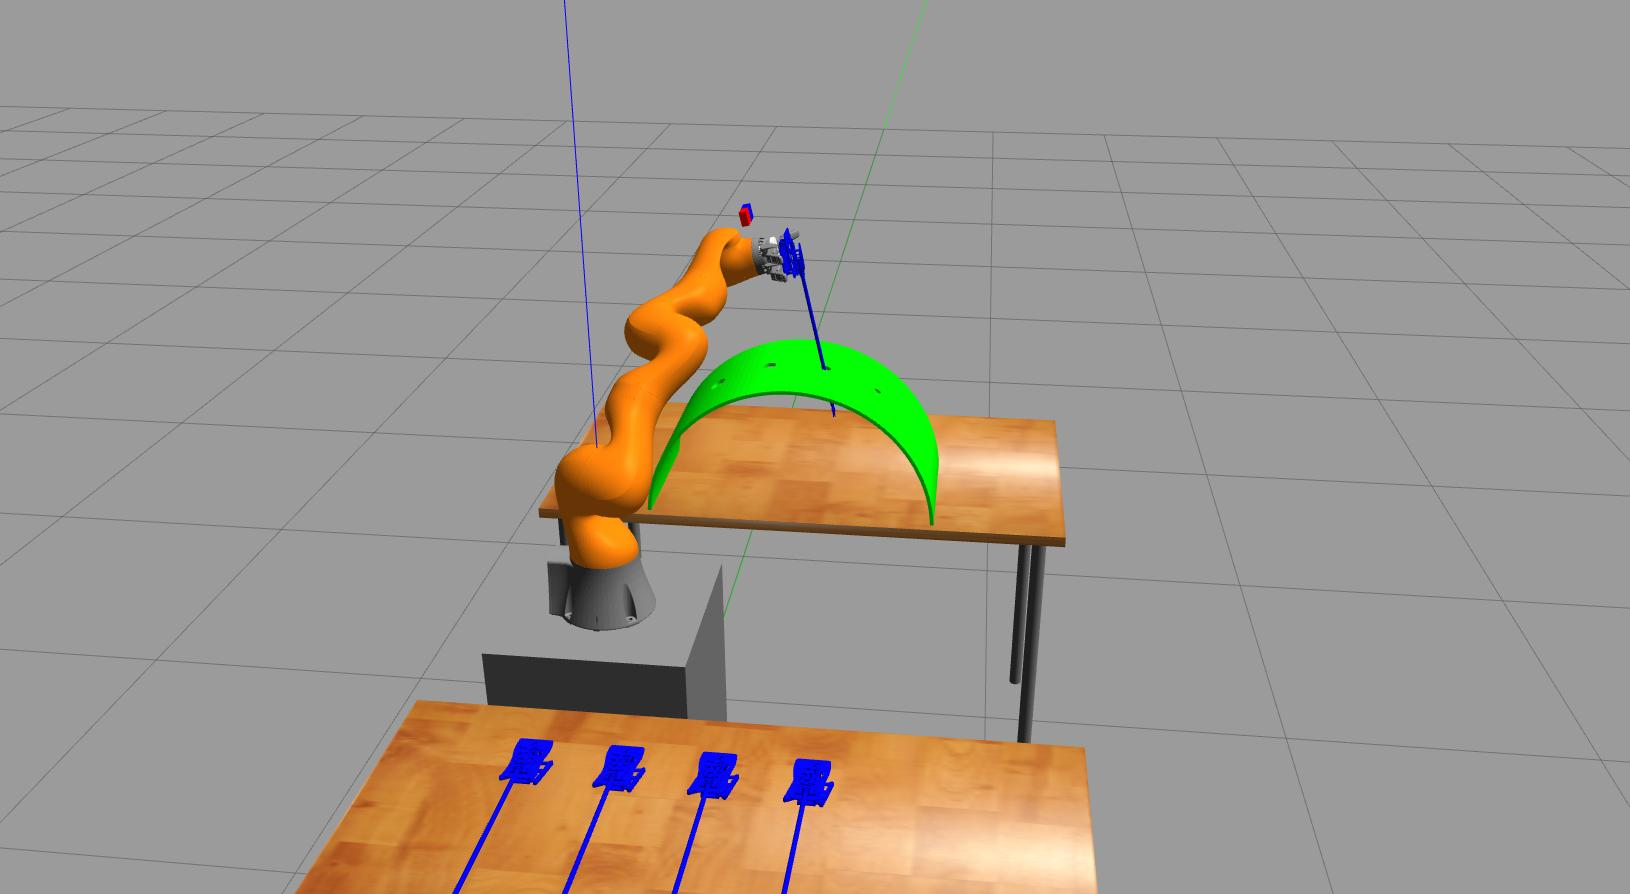
\includegraphics[width=0.3\textwidth]{../images/robot_planner2/robot_planner2_8}\\
\caption{Experiment 2a: first layout}
\label{experiment-robot-planner2a}
\end{figure}
\end{center}
\end{frame}


\begin{frame}
\frametitle{Robot Planner 2: Simulation layout and reachability experiments}
\begin{center}
\begin{figure}[!htb]
\centering
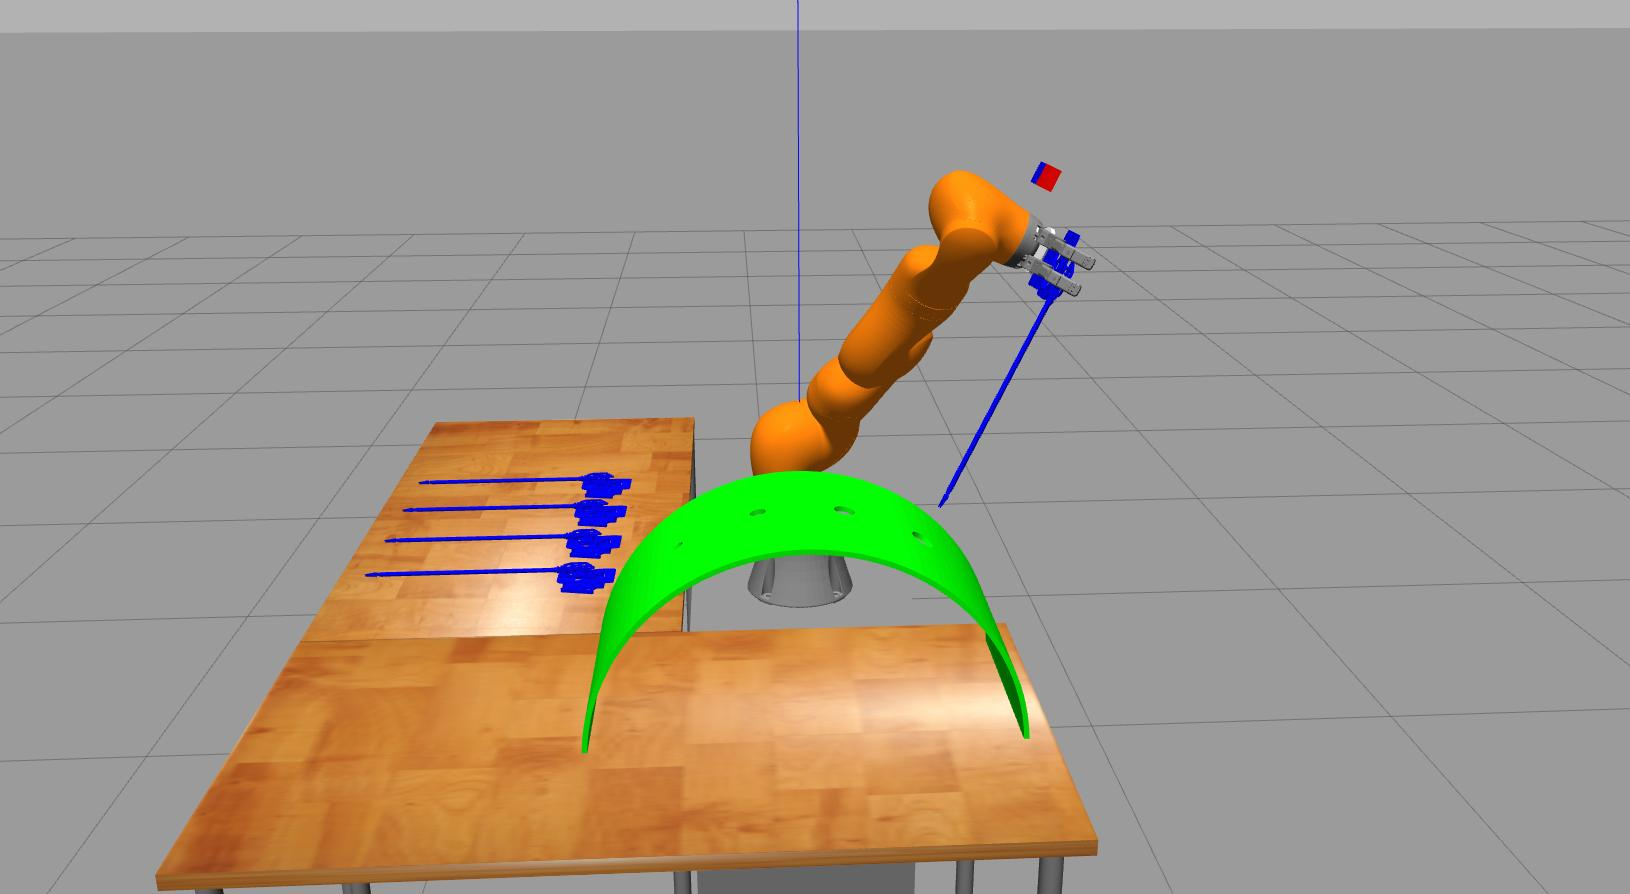
\includegraphics[width=0.3\textwidth]{../images/robot_planner2b/robot_planner2b_1}
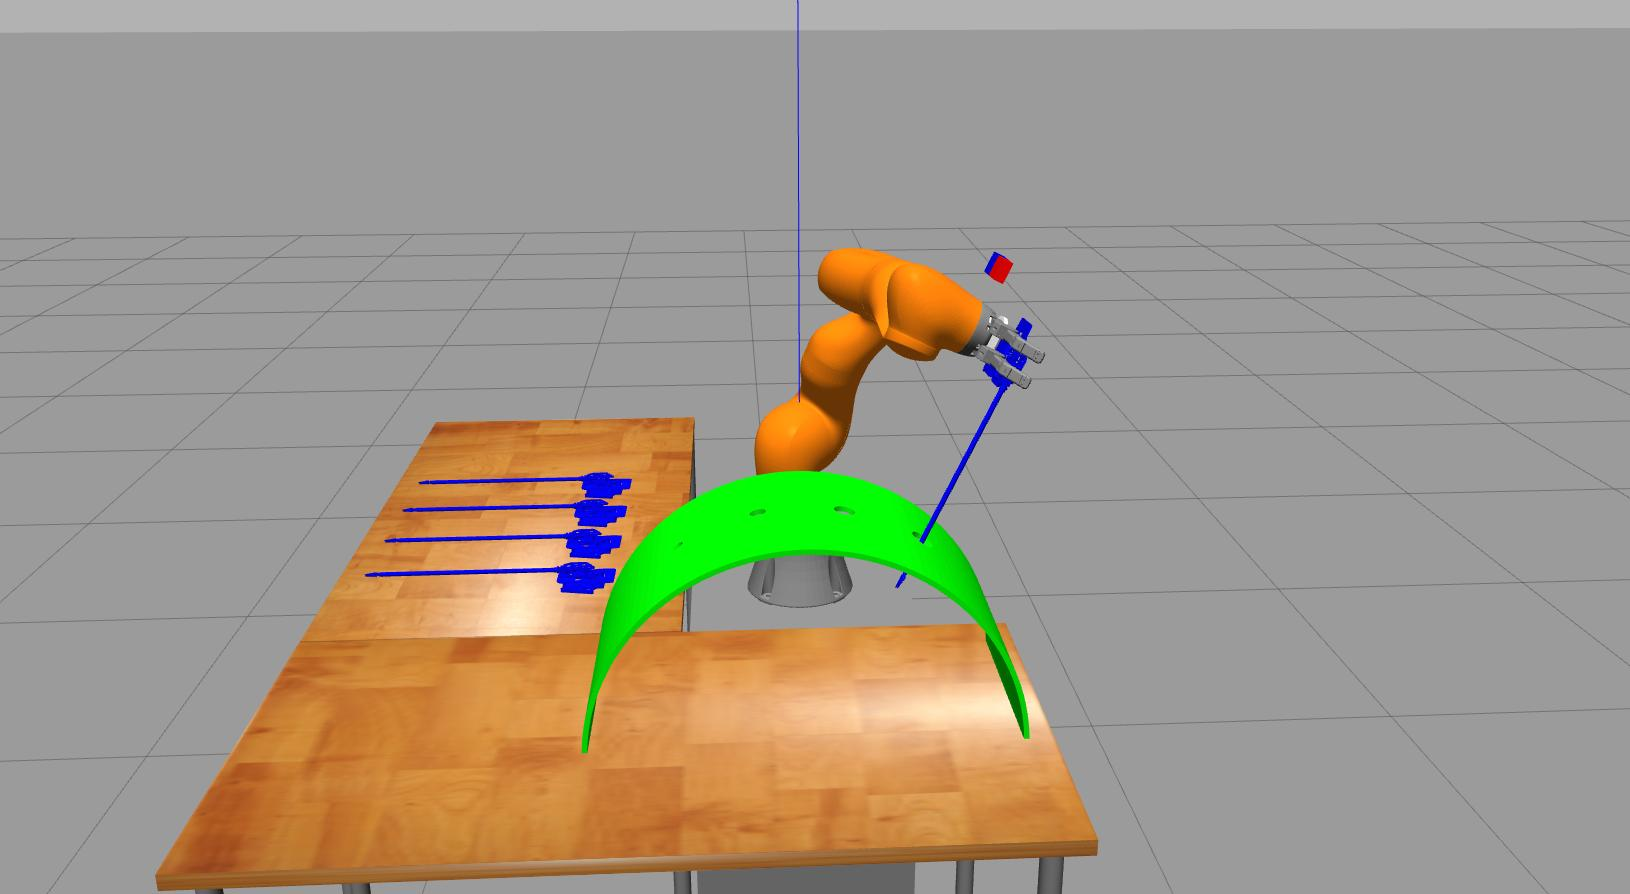
\includegraphics[width=0.3\textwidth]{../images/robot_planner2b/robot_planner2b_2}
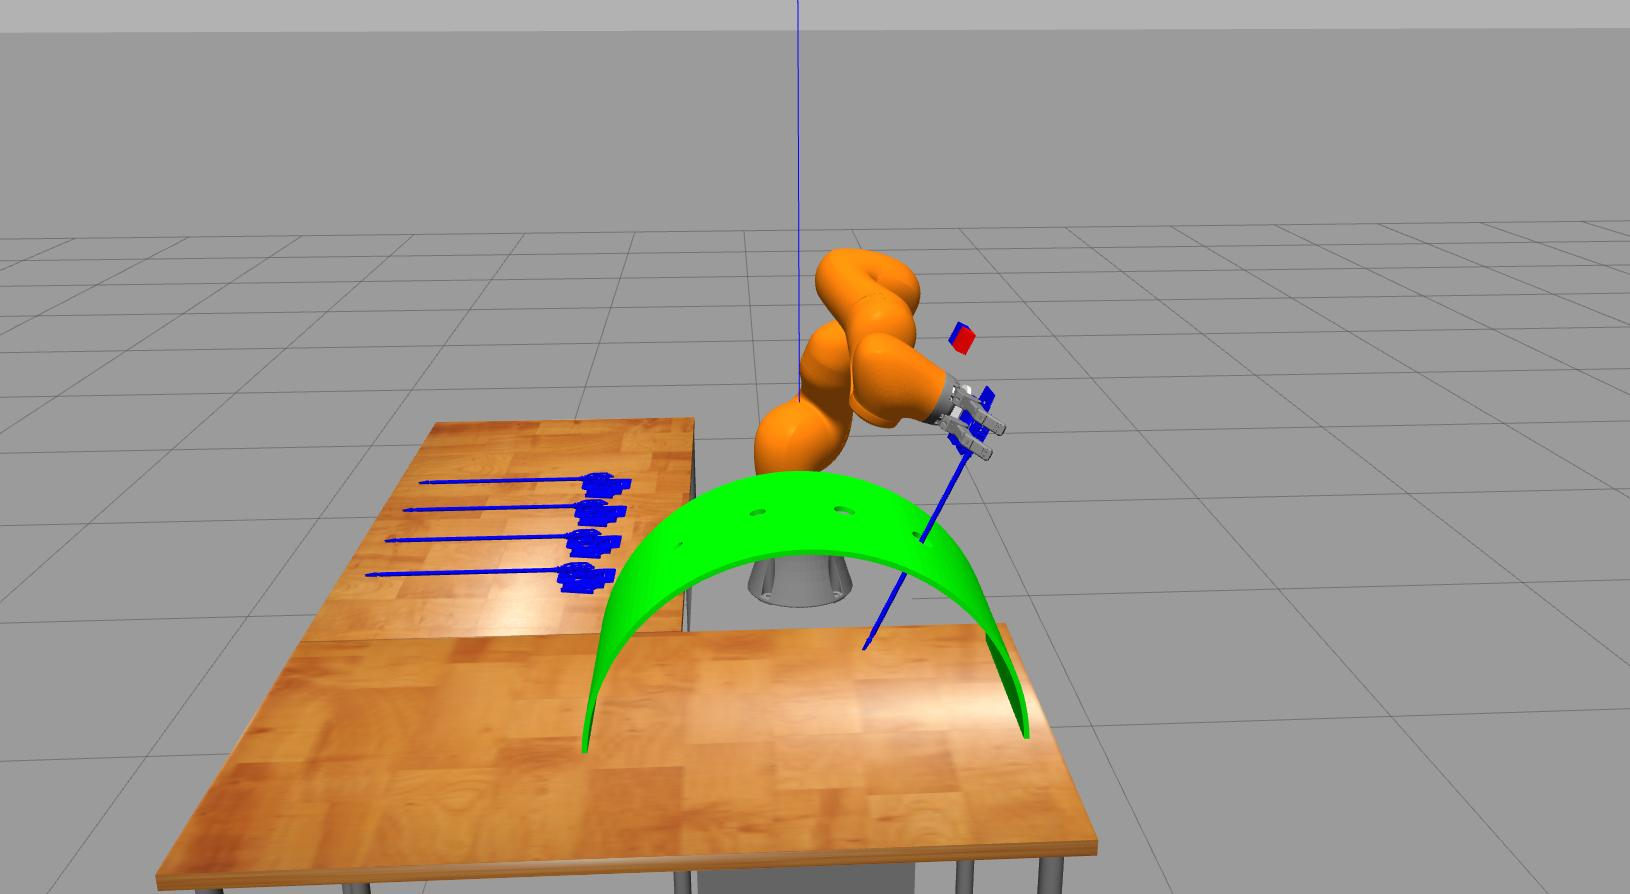
\includegraphics[width=0.3\textwidth]{../images/robot_planner2b/robot_planner2b_3}\\
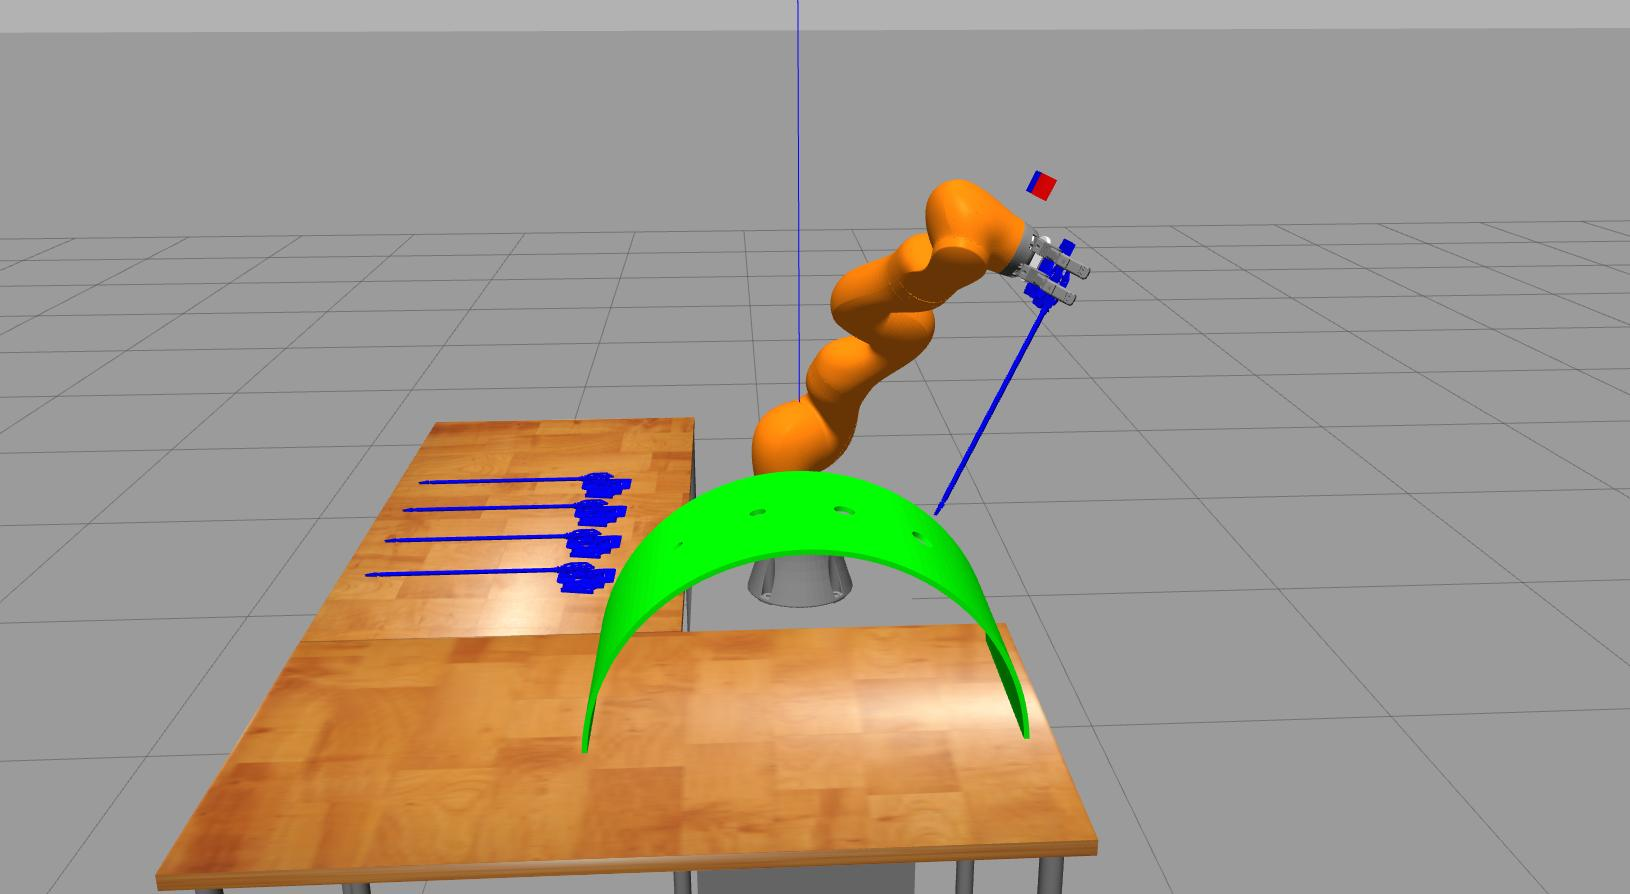
\includegraphics[width=0.3\textwidth]{../images/robot_planner2b/robot_planner2b_4}
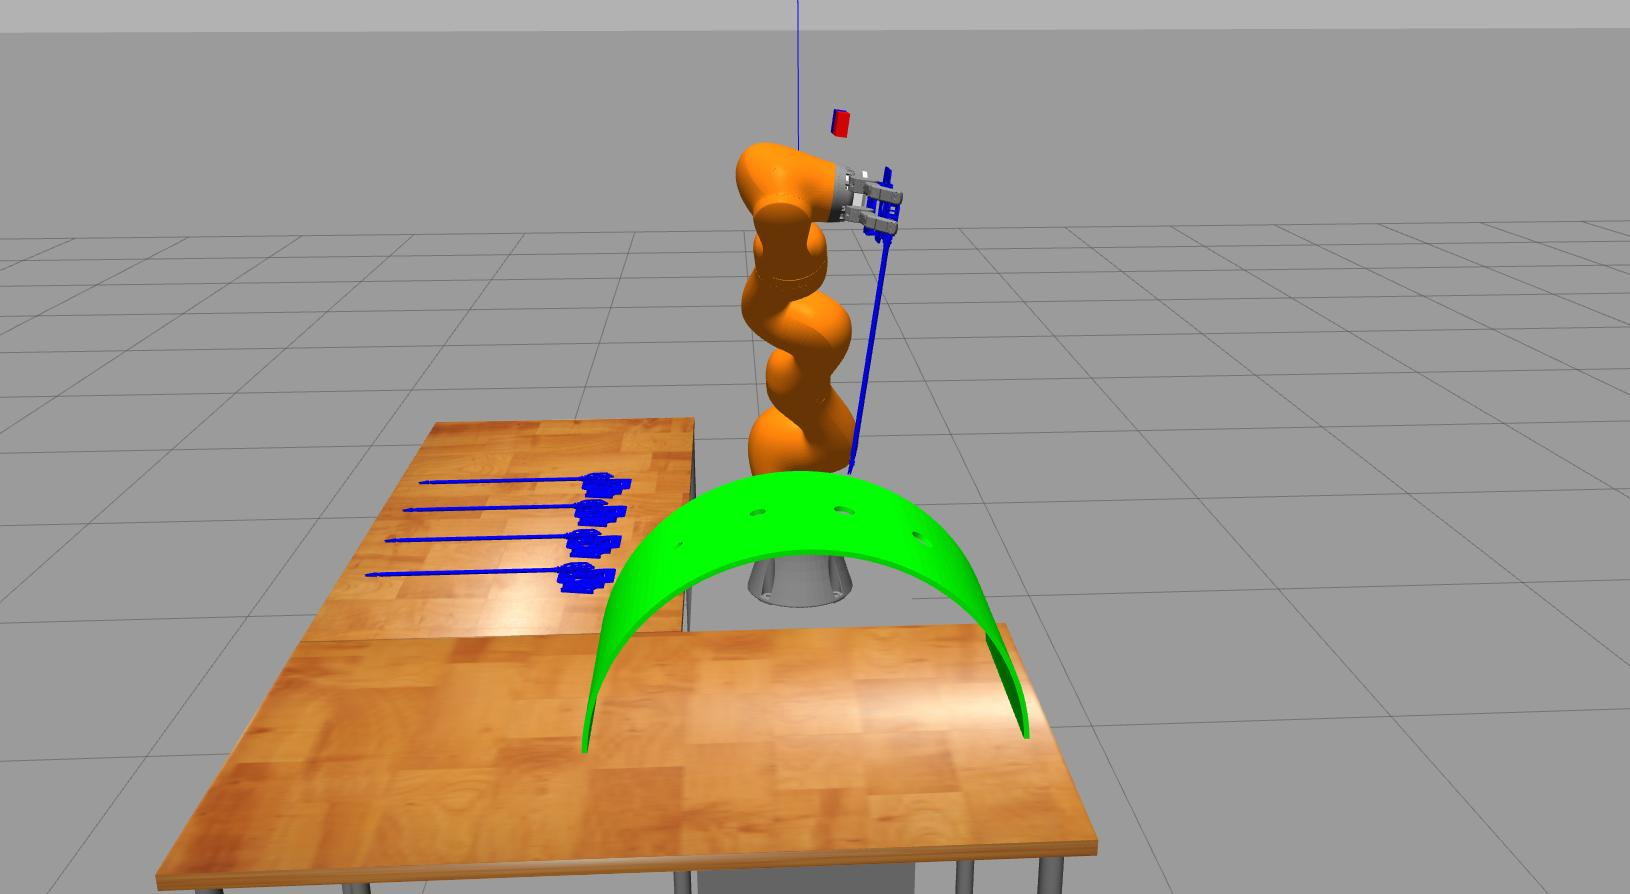
\includegraphics[width=0.3\textwidth]{../images/robot_planner2b/robot_planner2b_5}
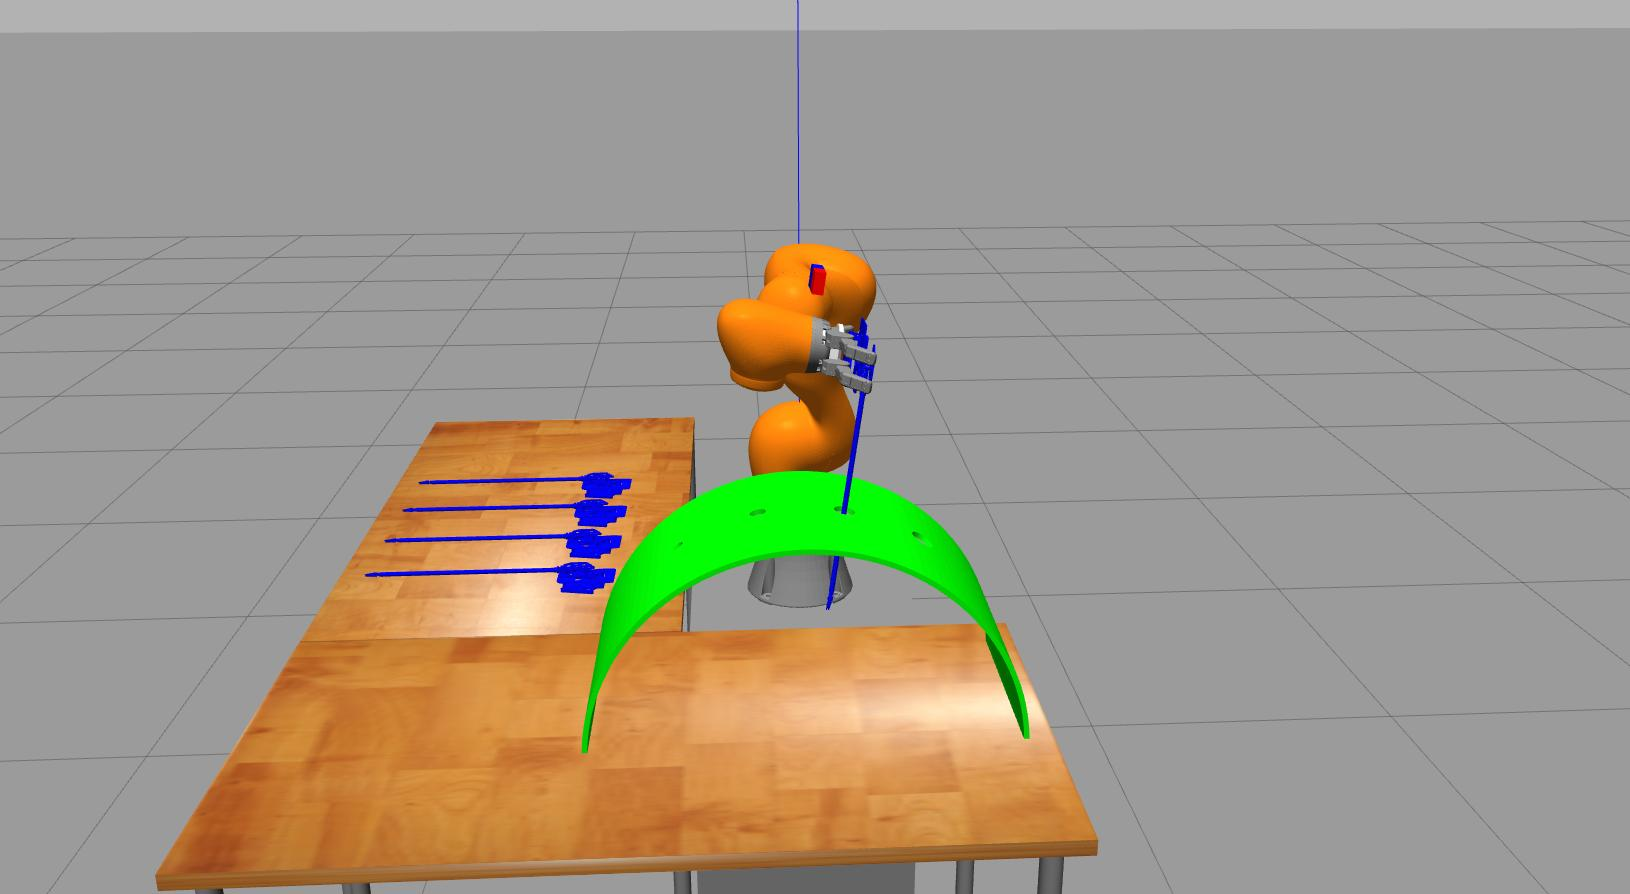
\includegraphics[width=0.3\textwidth]{../images/robot_planner2b/robot_planner2b_6}\\
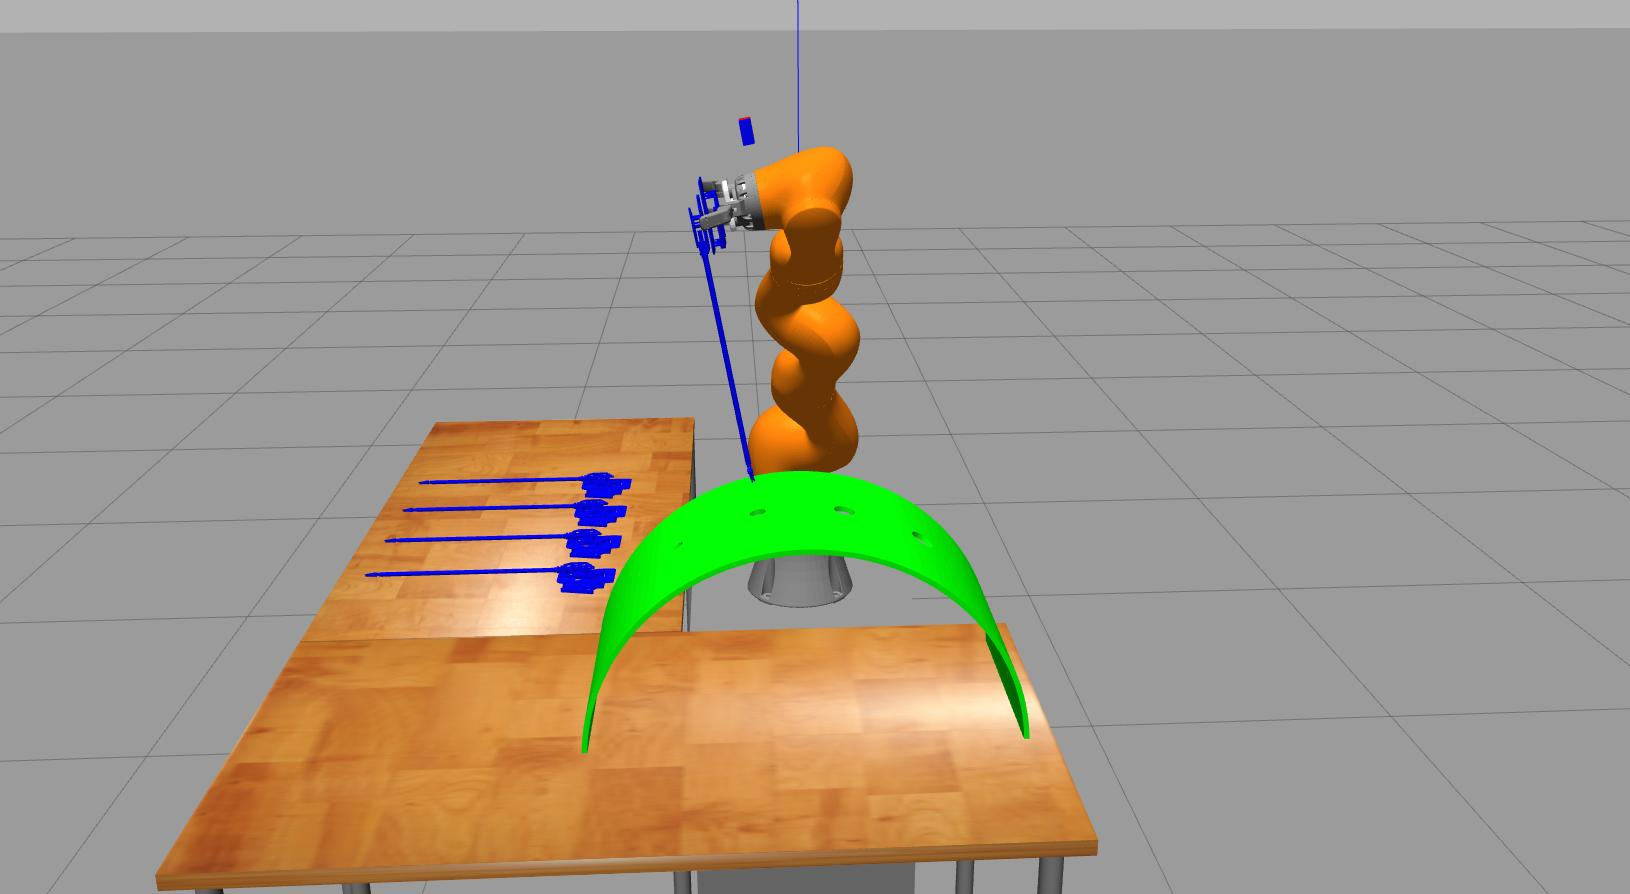
\includegraphics[width=0.3\textwidth]{../images/robot_planner2b/robot_planner2b_7}
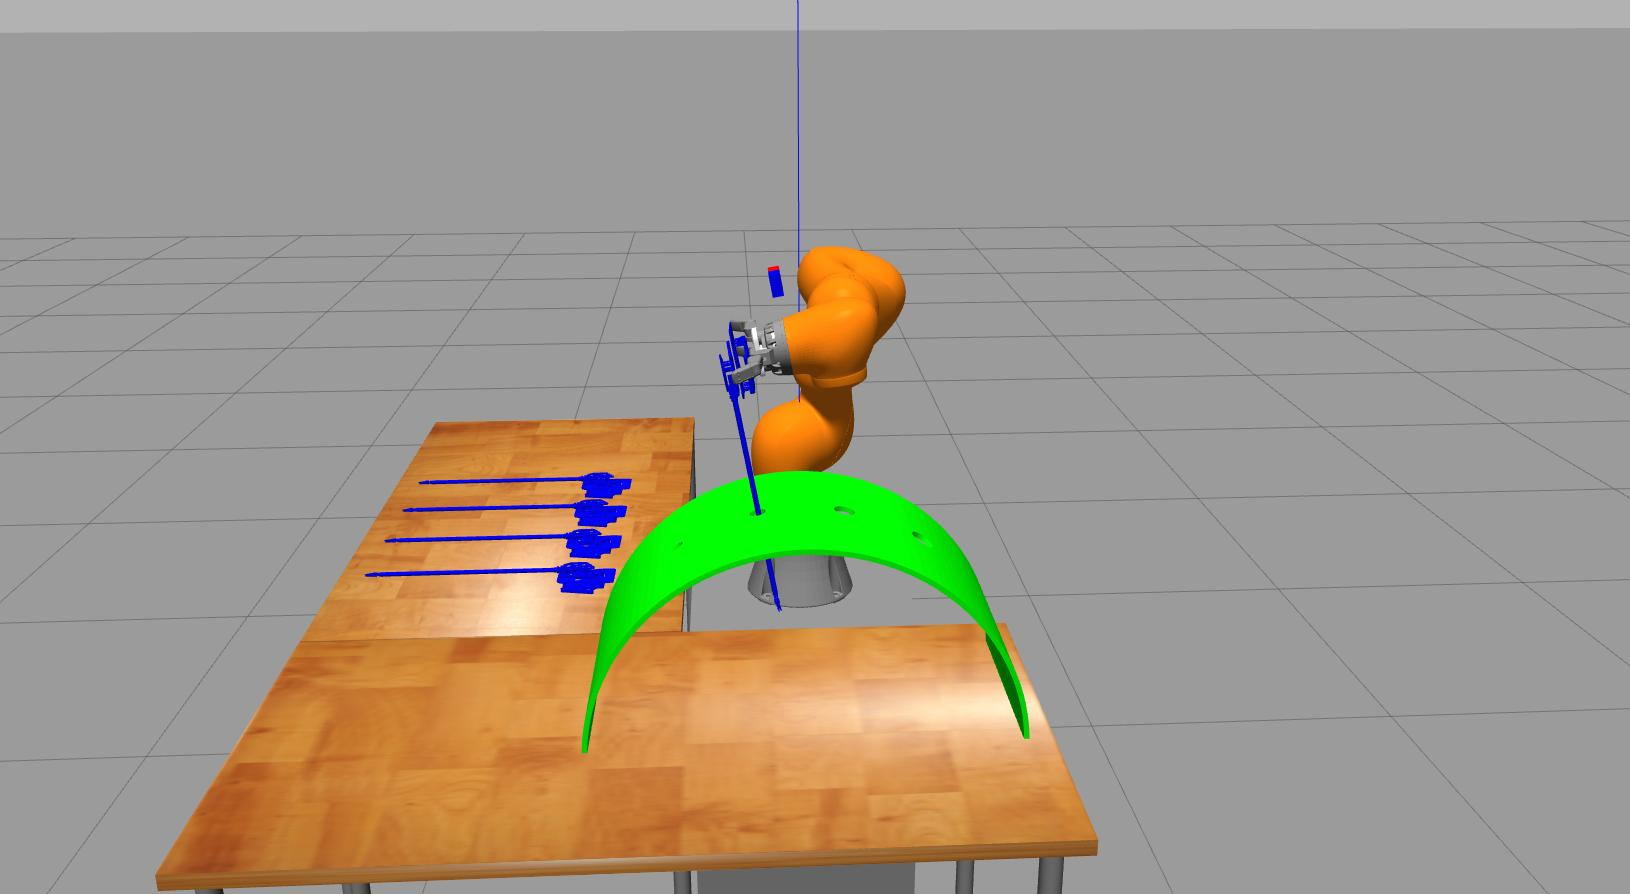
\includegraphics[width=0.3\textwidth]{../images/robot_planner2b/robot_planner2b_8}
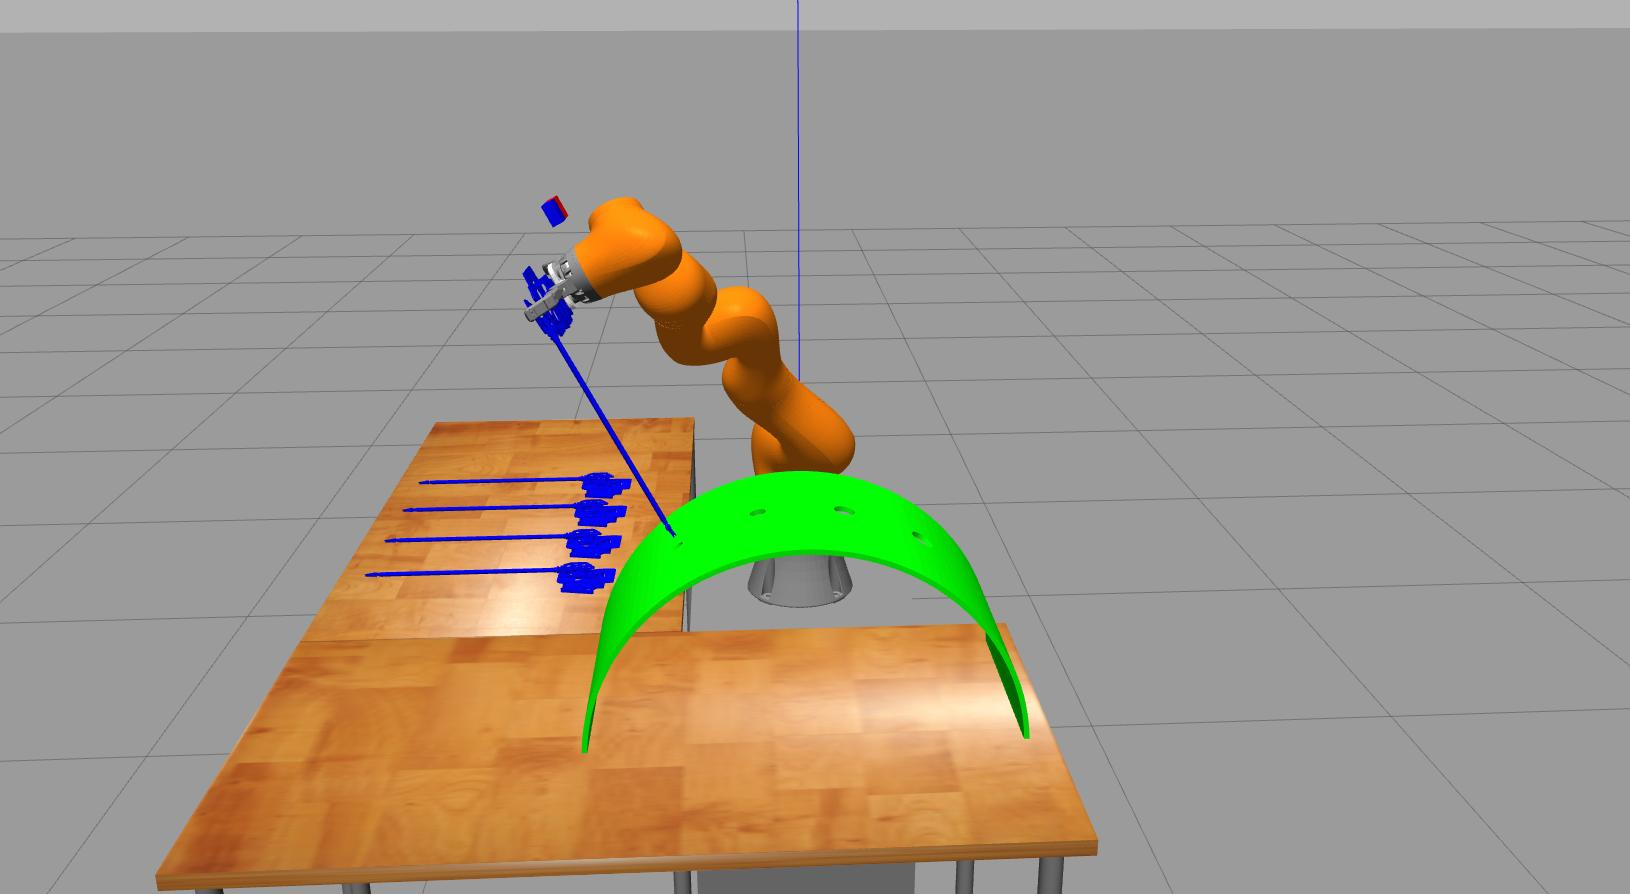
\includegraphics[width=0.3\textwidth]{../images/robot_planner2b/robot_planner2b_9}\\
\caption{Experiment 2b: second layout}
\end{figure}
\end{center}
\end{frame}


\begin{frame}
\frametitle{Robot Planner 3b: Line segment trajectories in task space}
\begin{center}
\begin{figure}[!htb]
\centering
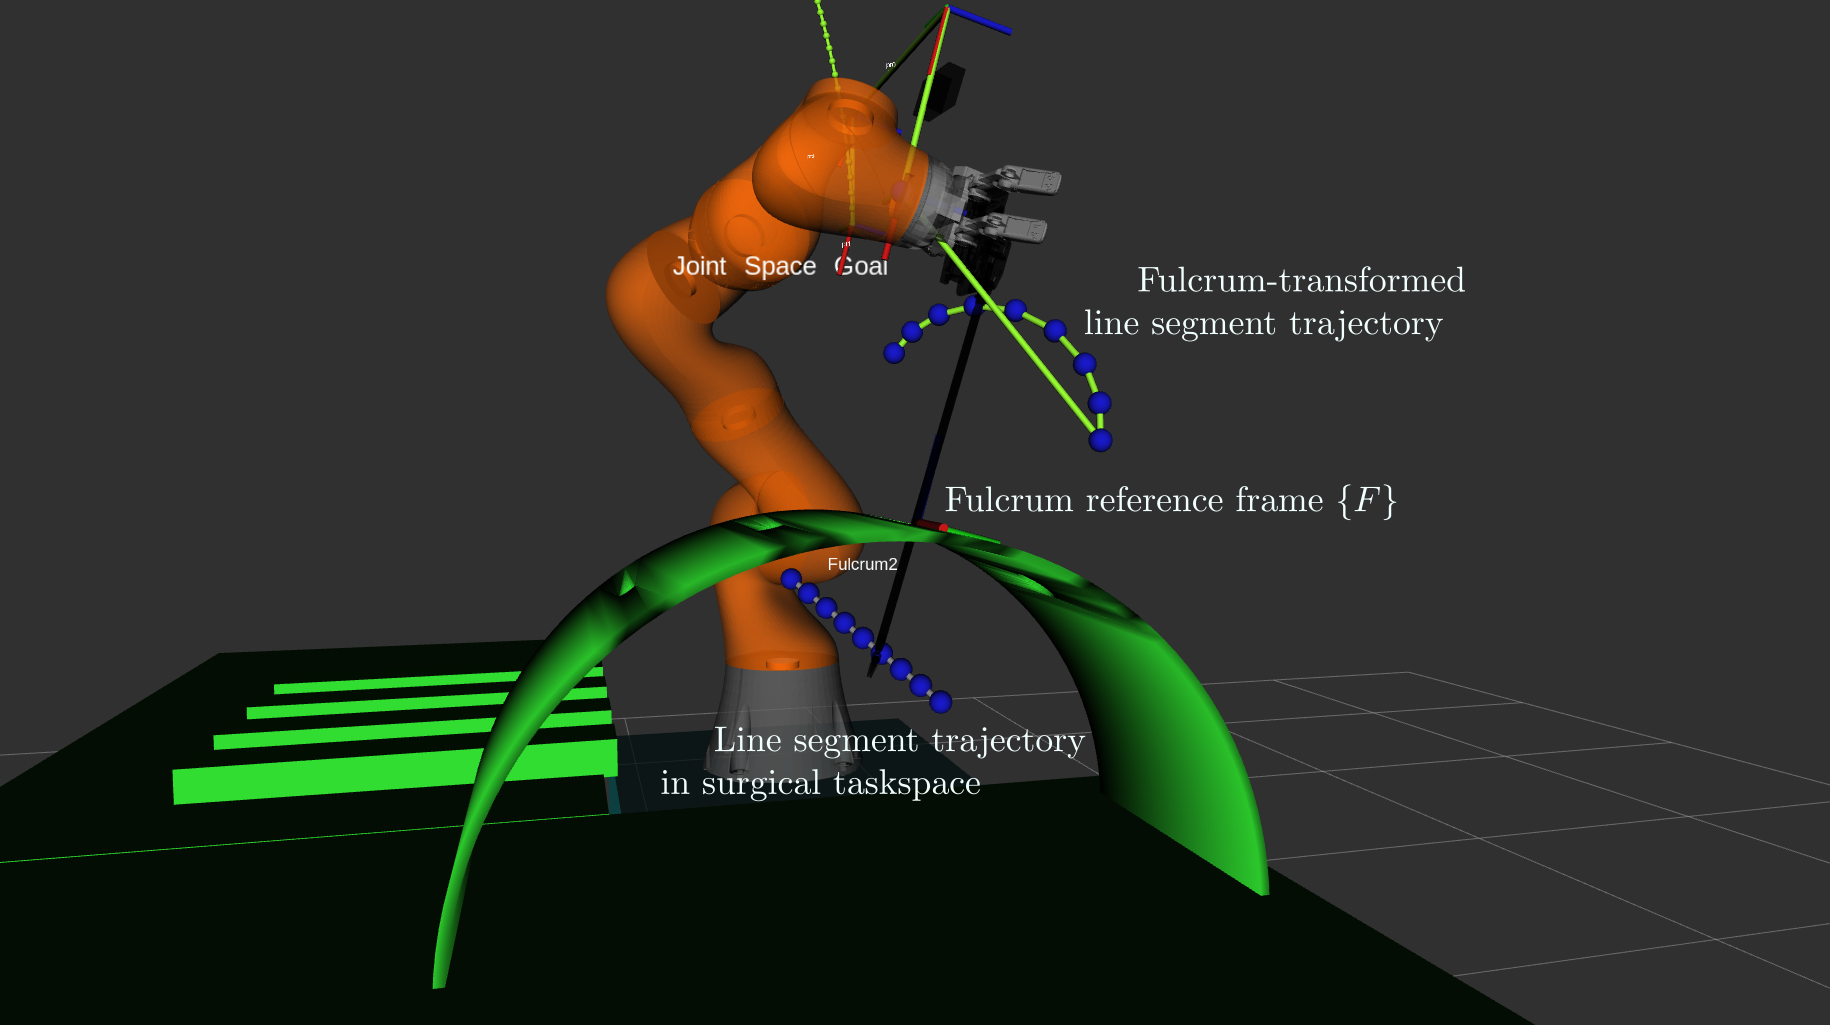
\includegraphics[width=0.9\textwidth]{../images/robot_planner3/3b_line_seg.png}
\caption{Experiment 3b}
\end{figure}
\end{center}
\end{frame}

\begin{frame}
\frametitle{Robot Planner 3b: Line segment trajectories in task space}
\begin{center}
\begin{figure}[!htb]
\centering
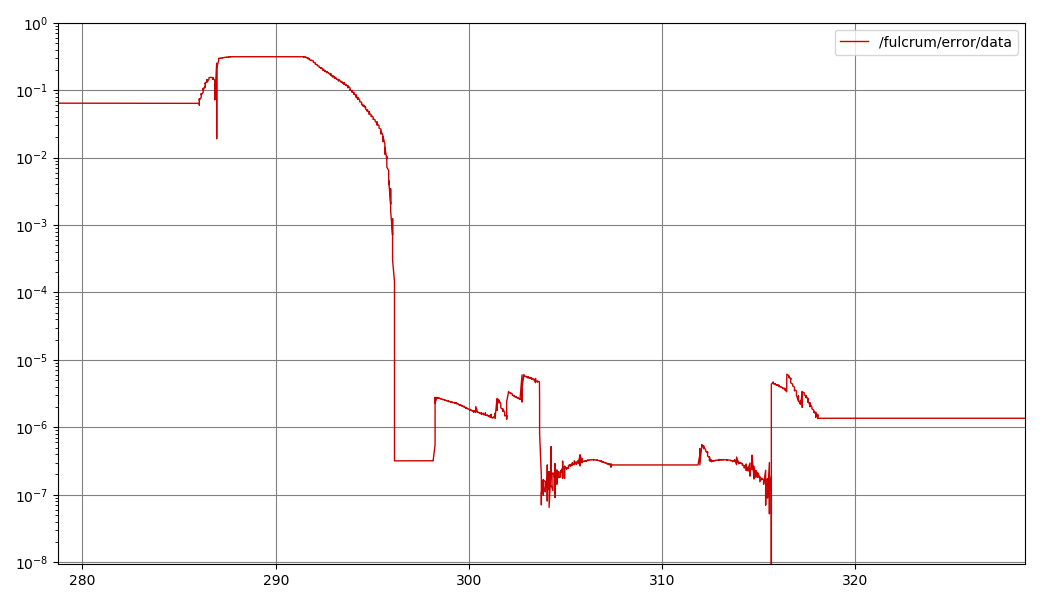
\includegraphics[width=0.8\textwidth]{../images/robot_planner3/robot_planner3b_error.png}
\caption{RCM error diagram from home position to line and reverse-line segment trajectories.}
\end{figure}
\end{center}
\end{frame}

\begin{frame}
\frametitle{Robot Planner 3b: Line segment trajectories in task space}
\begin{center}
\begin{figure}[!htb]
\centering
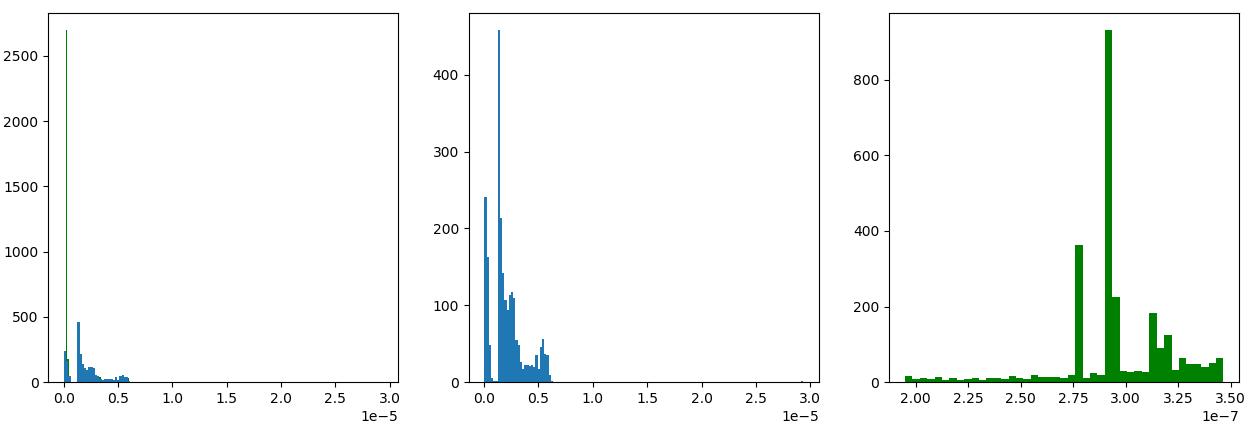
\includegraphics[width=0.8\textwidth]{../images/robot_planner3/robot_planner3b-error_distributions.png}
\caption{RCM error distributions, measurements from 10 iterations of the same experiment. From left to right: distribution of all measurements, distribution of measurements while the robot was pivoting, 
distribution of measurements while the robot was inserted but still.}
\end{figure}

\resizebox*{\textwidth}{!}{
\begin{tabular}{ |c|c|c|c| } 
\hline
 & Average [m] & Standard Deviation [m] & sample size \\
 & (accuracy) & (repeatability) & \\
\hline
\textbf{while pivoting} & $2.112649 \cdot 10^{-6}$ & $1.609277 \cdot 10^{-6}$ & 2309 \\
\hline
\textbf{while inserted and still} & $2.948652 \cdot 10^{-7}$ & $2.948652 \cdot 10^{-7}$ & 2696 \\
\hline
\end{tabular}
}
\end{center}
\end{frame}

\begin{frame}
\frametitle{Line segment trajectories in task space}
\begin{center}
\begin{figure}[!htb]
\centering
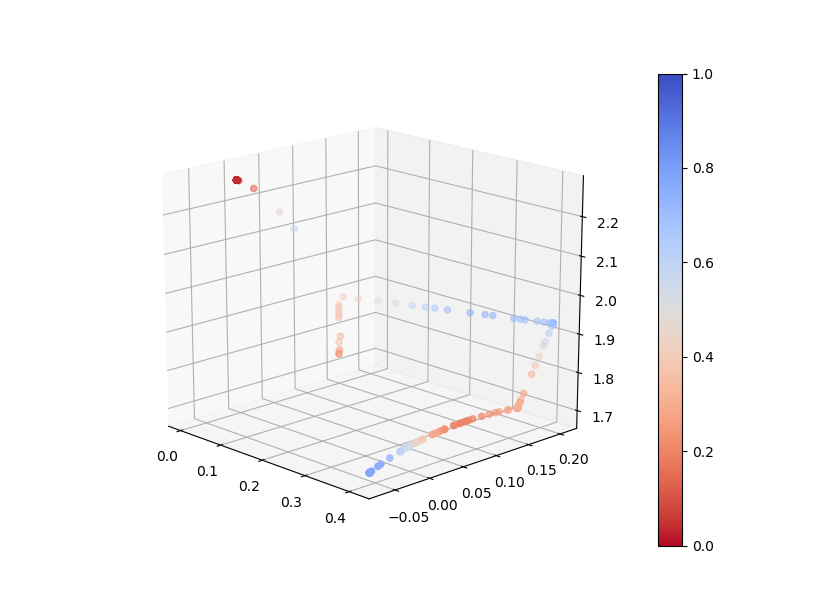
\includegraphics[width=0.49\textwidth]{../images/robot_planner3/robot_planner3b_manip1.png}
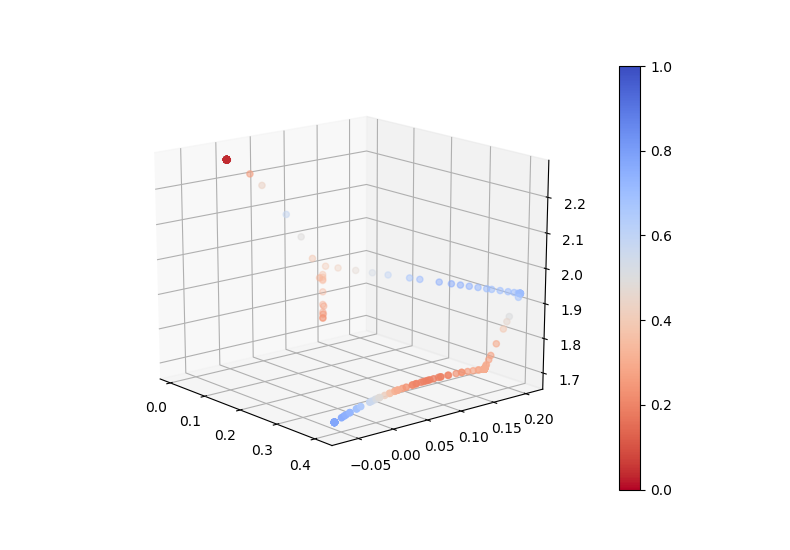
\includegraphics[width=0.49\textwidth]{../images/robot_planner3/robot_planner3b_manip2.png}
\caption{Experiment 3b: Manipulability plots of the whole trajectory the robot executed during 2 iterations of the same experiment}
\label{robot-planner3b-line-seg-manipulability-plots}
\end{figure}
\end{center}
\end{frame}

\begin{frame}
\begin{center}
\frametitle{Robot Planner 3b: Line segment trajectories in task space}
\resizebox{\textheight}{!}{
\begin{tabular}{ |p{0.2\textwidth}|p{0.2\textwidth}|p{0.2\textwidth}|p{0.2\textwidth}|p{0.2\textwidth}| } 
\hline
Robot Planner 3b          & \multicolumn{4}{c}{Approach and \textbf{line segment pivot} trajectories with \textbf{RRTConnect}}                                                                                                 \vline \\
\hline
                          & \multicolumn{4}{c}{\textbf{elbow-up preparatory path}}                     \vline \\
\hline
10 Experiments            & Elbow-up Start pose planning time (sec) & Execution status & Elbow-up preparation path planning time (sec) & Execution status  \\
\hline
\textbf{Average} & 0.174222 & 1 & 0.117040	& 1 \\
\hline
\textbf{Standard deviation} & 	0.049002 &	- &	0.084238 & - \\
\hline
                          & \multicolumn{4}{c}{\textbf{Approach \& Insertion}}                     \vline \\
\hline
10 Experiments            & Approach fulcrum 2 path planning time (sec) & Execution status & Insertion path planning time (sec) & Execution status  \\
\hline
\textbf{Average} & 0.116498 &	1 &	0.249556 &	1 \\
\hline
\textbf{Standard deviation} & 	0.088078 &	- &	0.078941 & - \\
\hline
                          & \multicolumn{4}{c}{\textbf{Line segment pivot trajectories}}                     \vline \\
\hline
10 Experiments            & Line segment path planning time (sec) & Execution status & Reverse line segment path planning time (sec) & Execution status  \\
\hline
\textbf{Average} & 1.809001 &	1 &	5.356607 &	0.7 \\
\hline
\textbf{Standard deviation} & 	2.421448 &	- &	0.086818 & - \\
\hline
\end{tabular}
}
\end{center}
\end{frame}


\begin{frame}
\frametitle{Robot Planner 3a: Circular and Circular arc trajectories in task space}
\begin{center}
\begin{figure}[!htb]
\centering
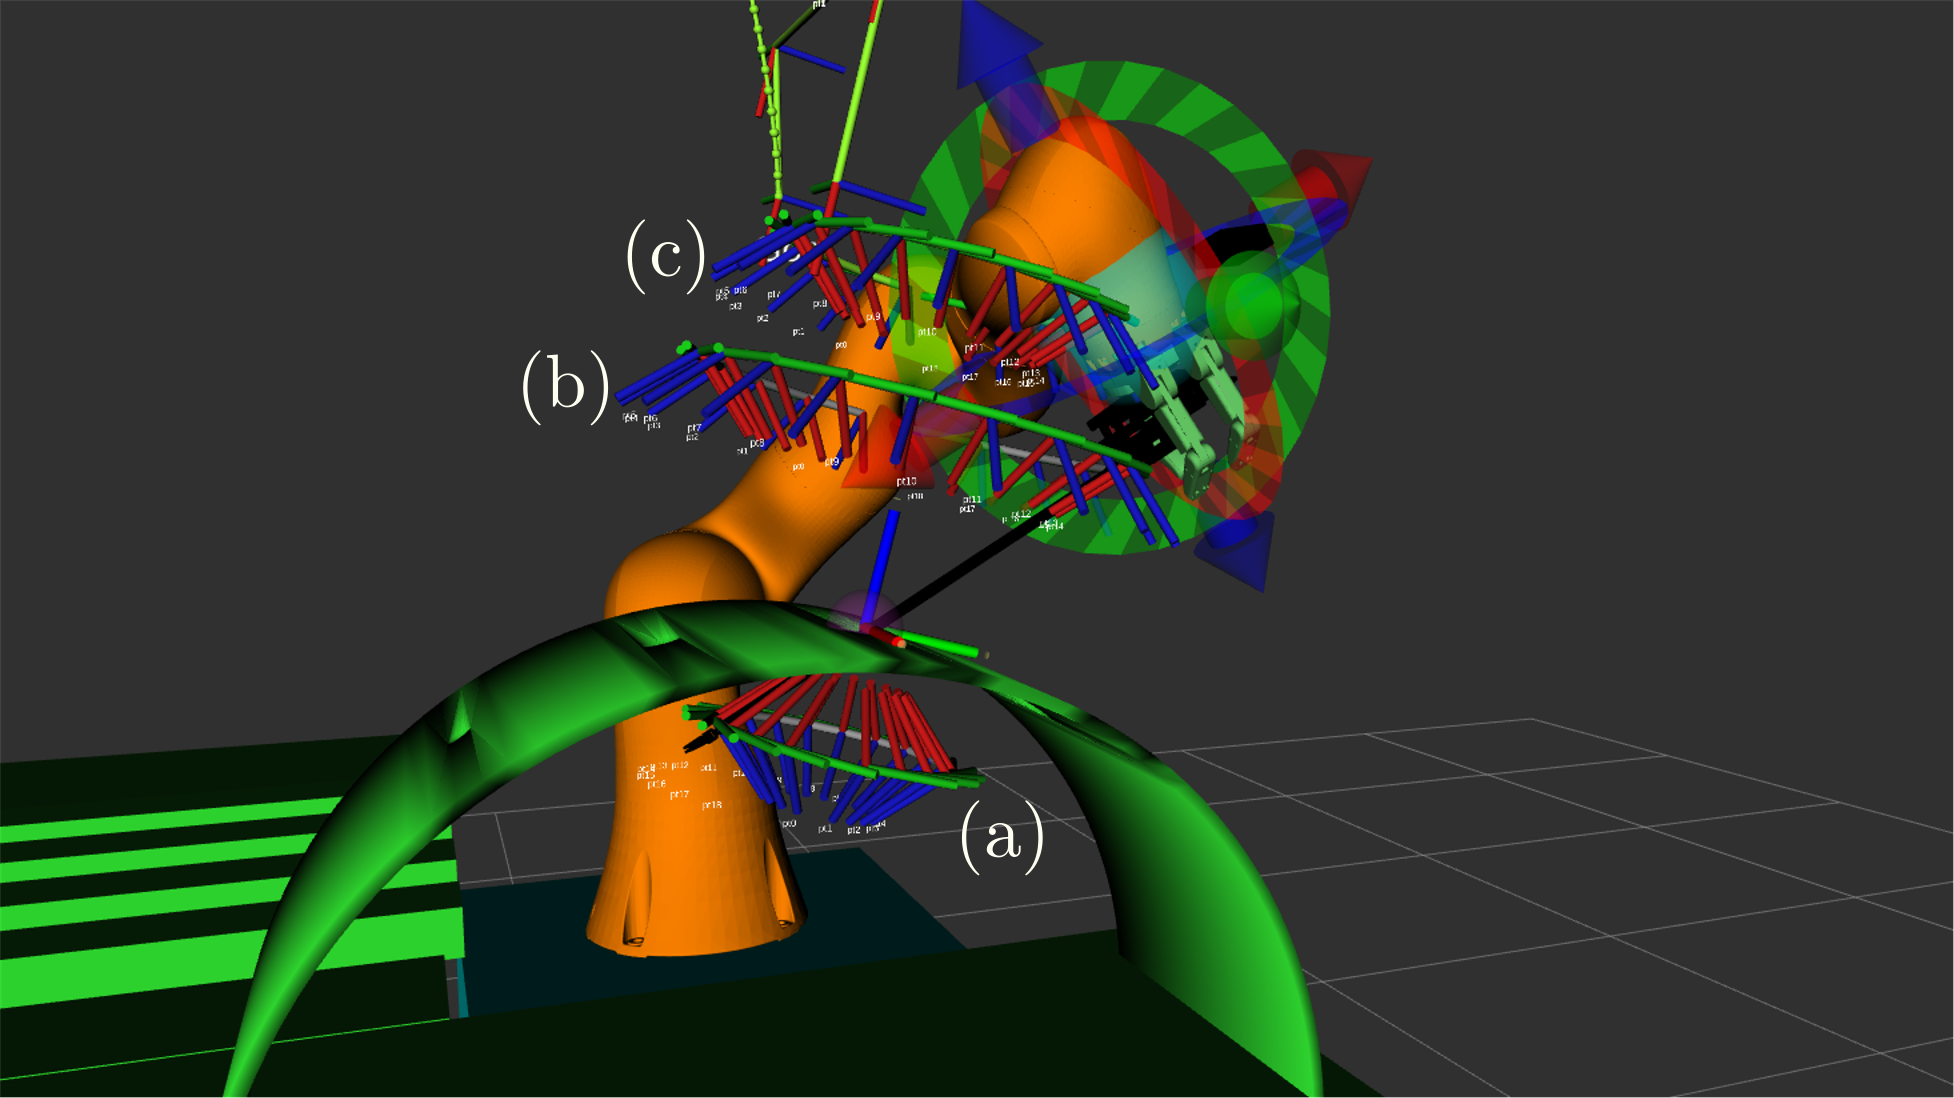
\includegraphics[width=0.8\textwidth]{../images/robot_planner3/3a_circle_details.png}
\caption{(a) The original circular trajectory designed inside the surgical taskspace, (b) the transformed trajectory that the base of the surgical tool will
 follow, (c) the actual transformed trajectory that the robot's end-effector will follow}
\label{robot-planner3a-circle-details}
\end{figure}
\end{center}
\end{frame}


\begin{frame}
\frametitle{Robot Planner 3h: Helical trajectories in task space}
\end{frame}

\begin{frame}
\frametitle{Robot Planner 4: Simple cube pick-and-place experiment}
\end{frame}

\begin{frame}
\frametitle{Robot Planner 5: Visual servoing}
\begin{center}
\begin{figure}[!htb]
\centering
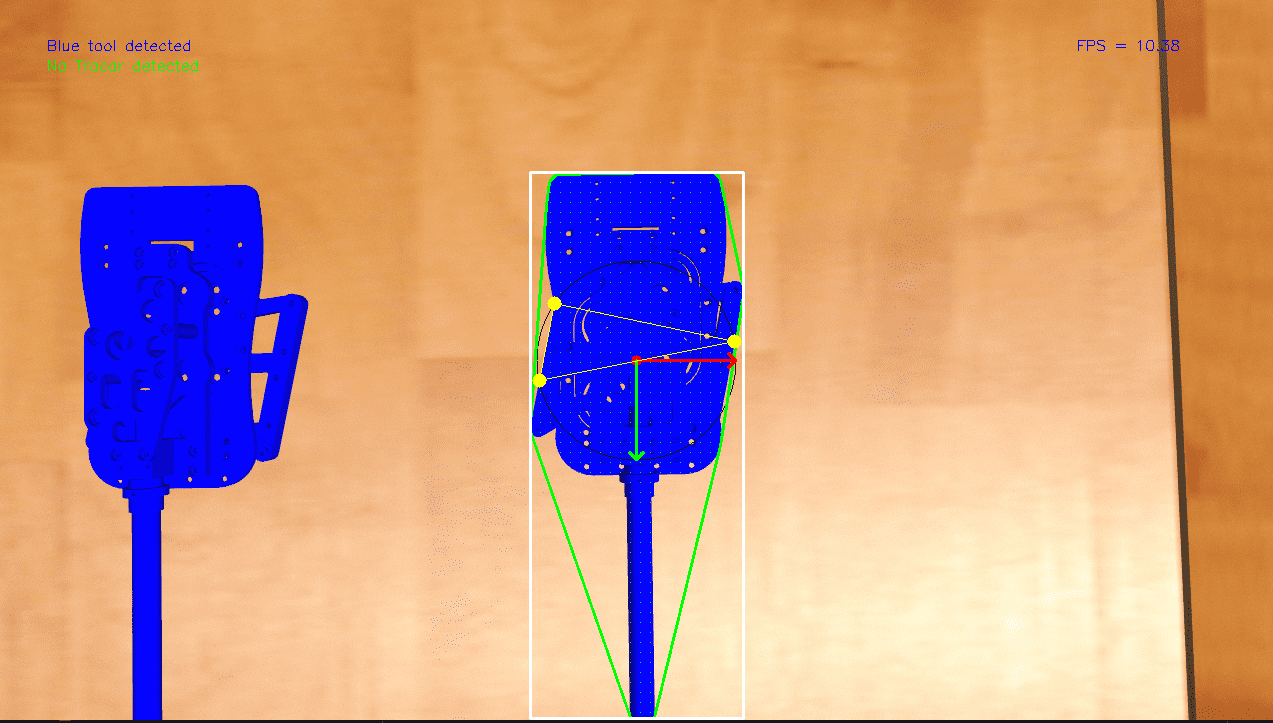
\includegraphics[width=0.6\textwidth]{../images/grasp-points-triangle.png}\\
\caption{Image based visual servoing and calculation of grasp points. The yellow points are the grasp points and the thin black circumscribed circle is the growing circle that was used to calculate them.}
\end{figure}
\end{center}
\end{frame}

\begin{frame}
\frametitle{Robot Planner 5: Visual servoing}
\begin{center}
\begin{figure}[!htb]
\centering
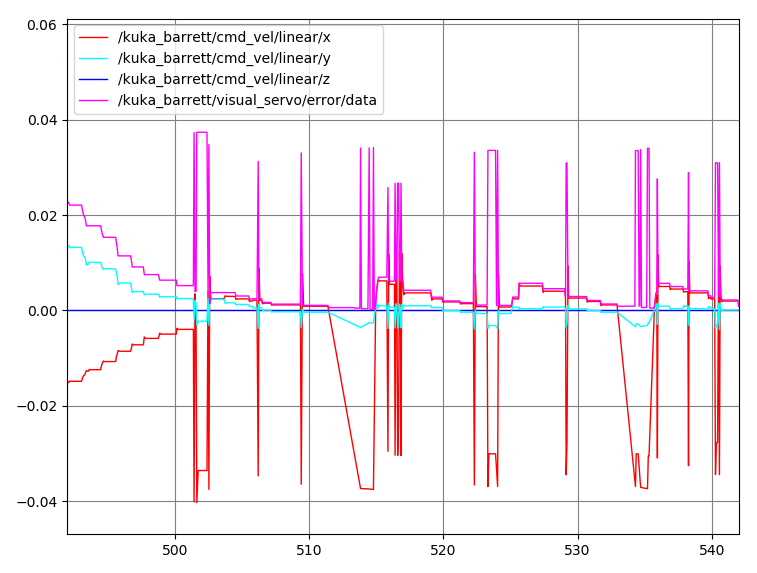
\includegraphics[width=0.45\textwidth]{../images/robot_planner5/visual_servo_controller3.png}
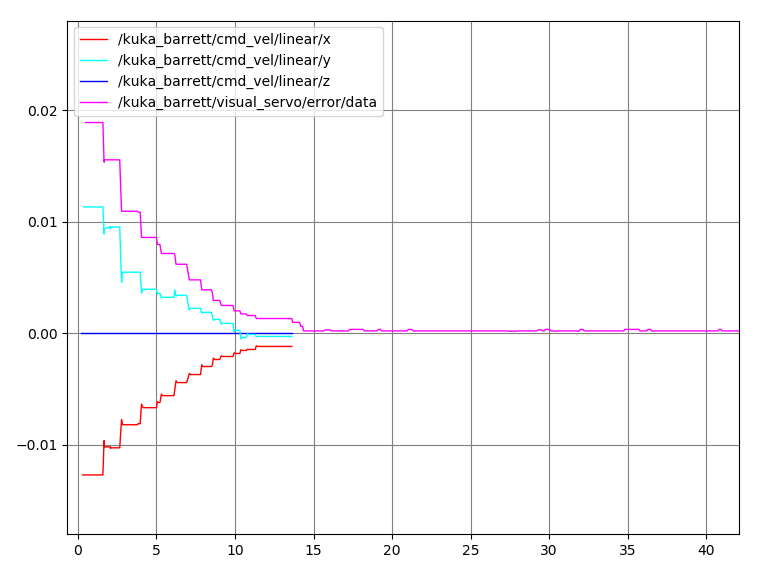
\includegraphics[width=0.45\textwidth]{../images/robot_planner5/visual_servo_controller4.png}\\
\caption{Visual servo controller error diagrams. On the left image in the error graphs appear some spikes. These spikes occur from the sudden temporary detection 
of a nearby surgical tool. On the right image, these spikes are filtered out, and only the error graphs of the visual servoing of one tool are shown. The  
controller parameters are $K_p = 0.9, K_d = 0.2$}
\end{figure}
\end{center}
\end{frame}

\begin{frame}
\frametitle{Robot Planner 6: RCM alignment error in insertion and retraction}
\end{frame}

\begin{frame}
\frametitle{Robot Planner 7: State machine - End-to-end simulation}

\begin{columns}

\column{0.6\textwidth}
\begin{center}
\begin{figure}[!htb]
\centering
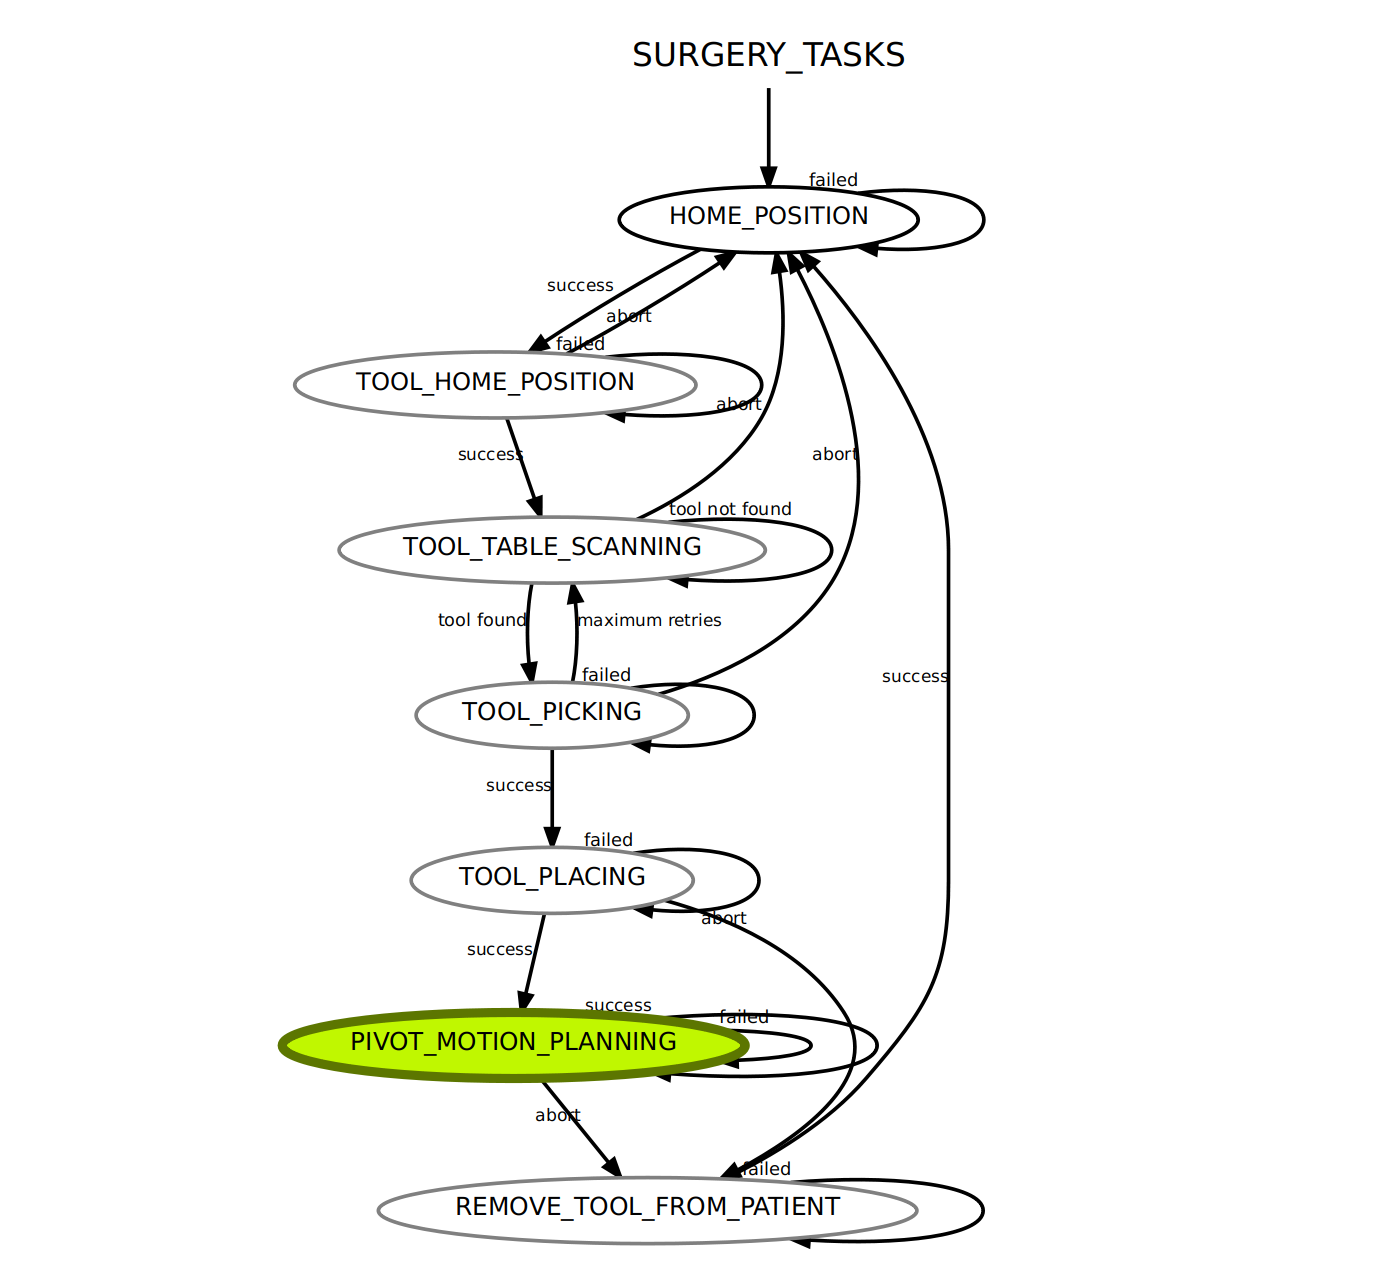
\includegraphics[width=\textwidth]{../images/state-machine-all-tasks.png}
\label{smack-state-machine}
\end{figure}
\end{center}

\column{0.3\textwidth}
Run all the stages of this thesis together (integration testing) using a state machine.
\end{columns}
\end{frame}


\begin{frame}
\frametitle{Demo}
\begin{center}
\begin{figure}[!htb]
\centering
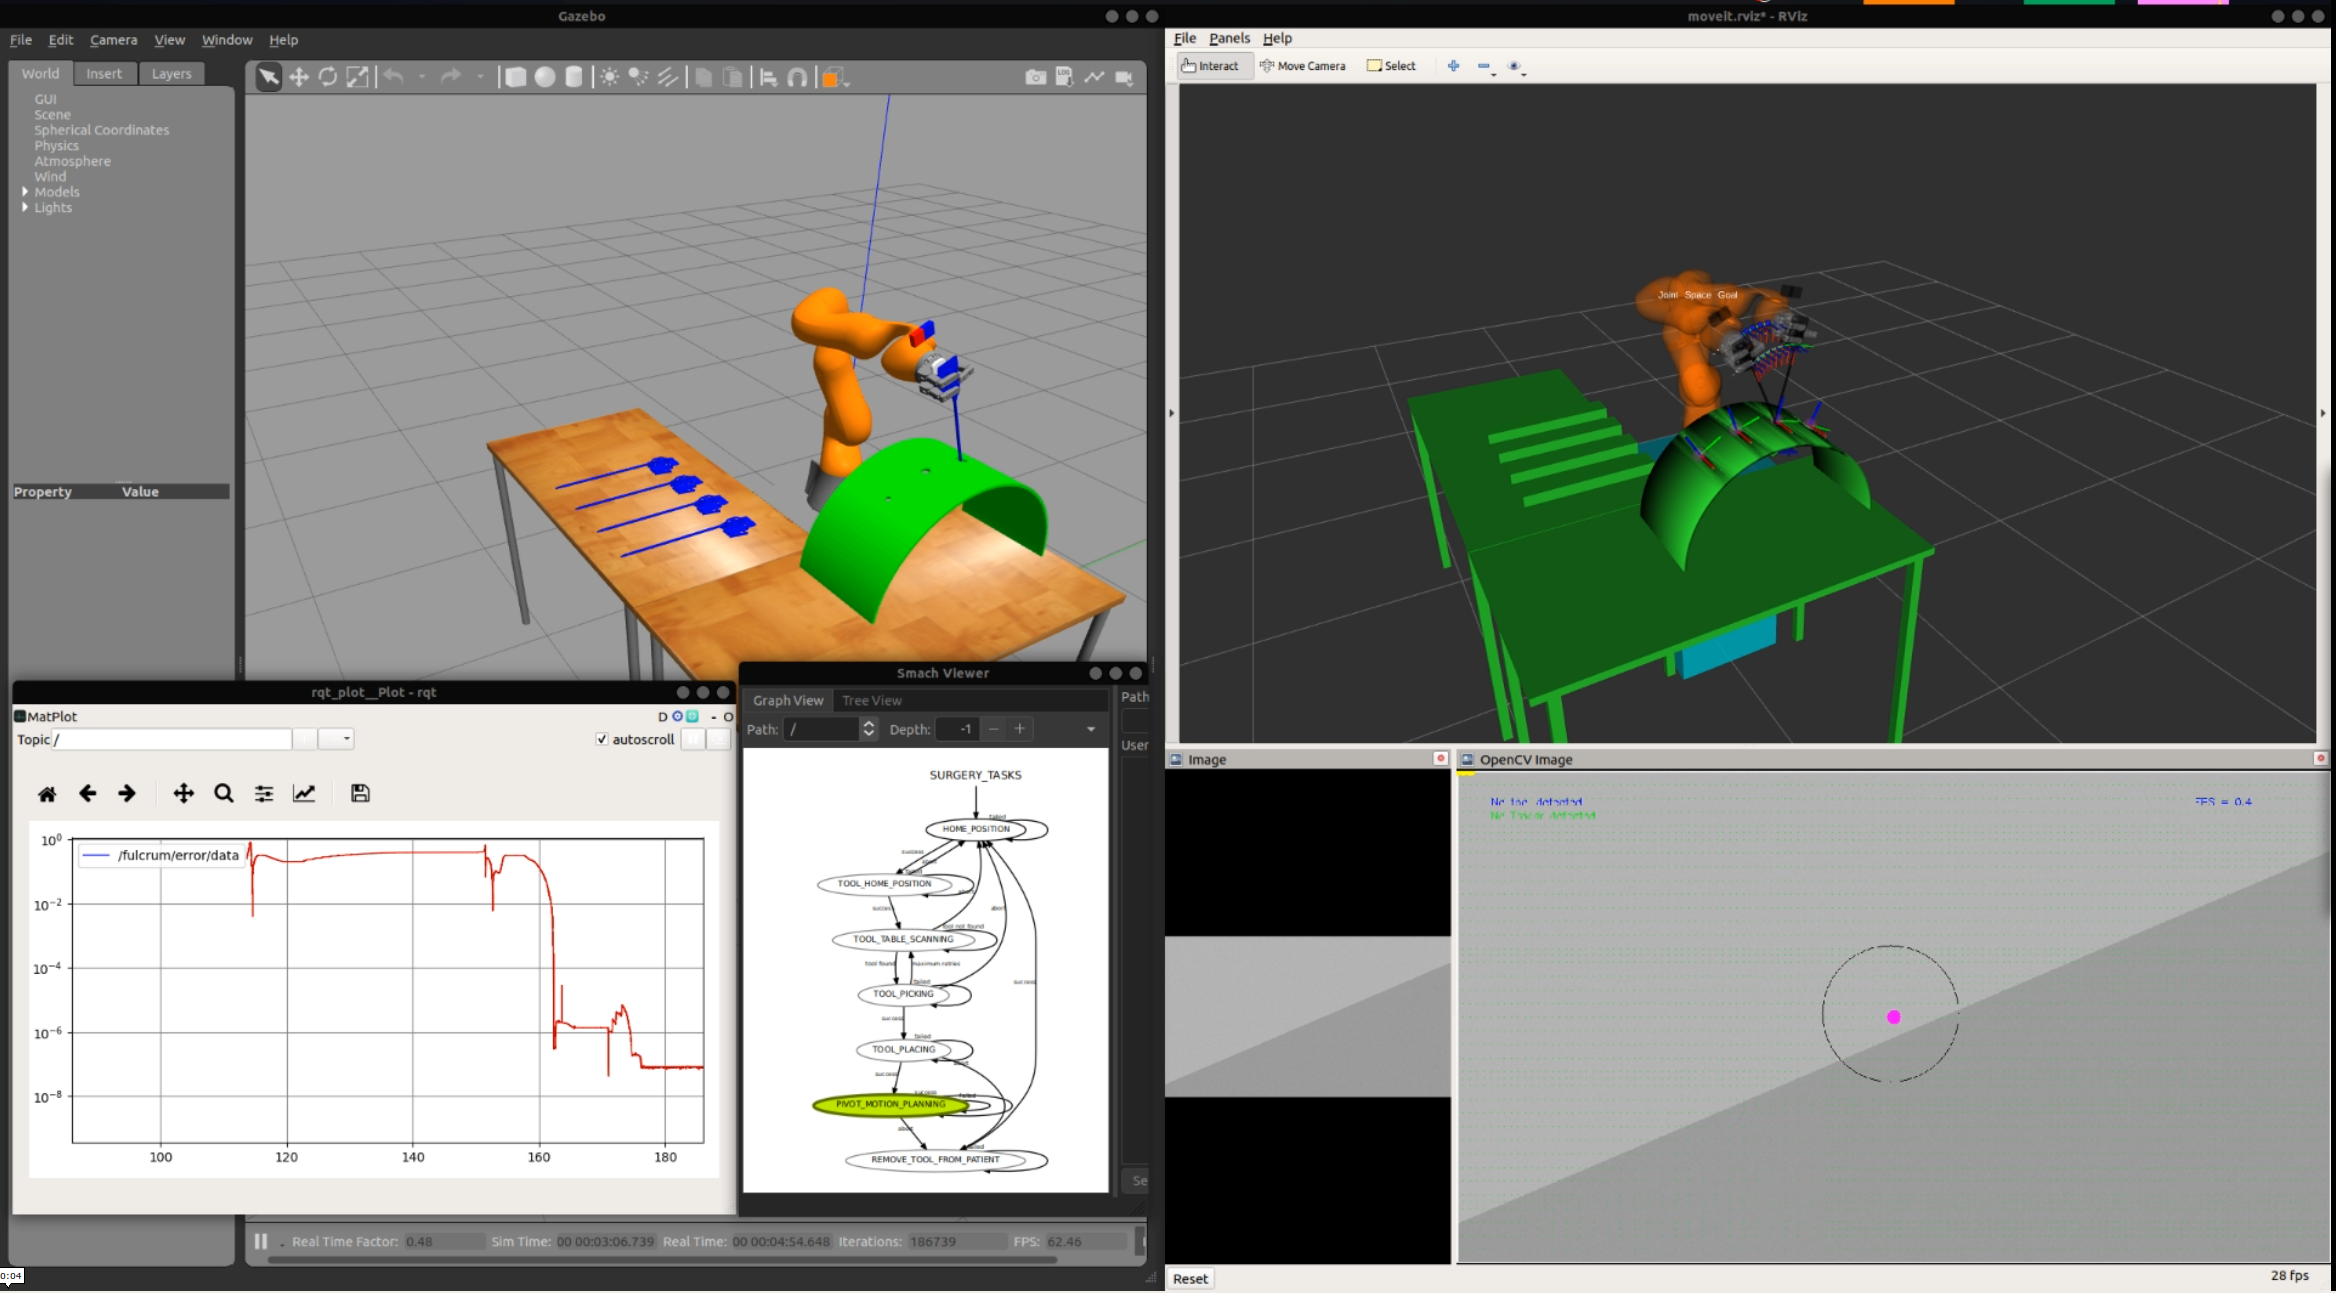
\includegraphics[width=\textwidth]{../images/demo.png}\\
\end{figure}
\url{https://youtu.be/lfV1vdHf7bk}
\end{center}
\end{frame}
